\documentclass{article}
\usepackage[utf8]{inputenc}
\usepackage{authblk}

\title{Software engineering 2}
\author[1]{Saman Fekri}
\author[2]{Parniya Saeedzadeh}
\date{November 2020}

\usepackage{natbib}
\usepackage{graphicx}

\usepackage[table,xcdraw]{xcolor}
\definecolor{tableBorderColor}{rgb}{.58,.66,.84}
\definecolor{tableHighlightColor}{rgb}{.85,.89,.95}
\definecolor{purpleHiglight}{rgb}{.63,.63,.76}
\definecolor{pinkHighlight}{rgb}{.95,.77, .88}

\usepackage{tabularx}
\usepackage{longtable}

\usepackage{float} 

\usepackage{caption}
\captionsetup[figure]{labelfont={bf},labelformat={default},labelsep=period,name={Figure}, font={scriptsize,it}}
\usepackage{subfig}
\usepackage{float}

\usepackage[a4paper,bindingoffset=0.2in,%
            left=1in,right=1in,top=1in,bottom=1in,%
            footskip=.25in]{geometry}

\usepackage{hyperref}
\usepackage{multirow}

\usepackage{listings}
\usepackage{enumitem}

\begin{document}


% \maketitle

% \section{Introduction}
% There is a theory which states that if ever anyone discovers exactly what the Universe is for and why it is here, it will instantly disappear and be replaced by something even more bizarre and inexplicable.
% There is another theory which states that this has already happened.\\
% ccadcdc 
% \begin{figure}[h!]
% \centering
% 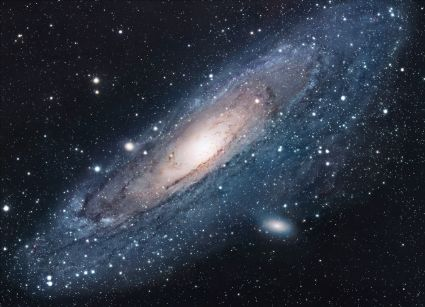
\includegraphics[scale=1.7]{universe}
% \caption{The Universe}
% \label{fig:universe}
% \end{figure}

% \section{Conclusion}
% ``I always thought something was fundamentally wrong with the universe'' \citep{adams1995hitchhiker}
% 
% \bibliographystyle{plain}
% \bibliography{references}

\begin{titlepage}

	\center % Centre everything on the page

	%------------------------------------------------
	%	Logo
	%------------------------------------------------
    \begin{figure}[H]
      \centering
      
\includegraphics[width=0.5\textwidth,keepaspectratio]{images/PolimiLogo1.png}
    \end{figure}
    
	\textsc{\LARGE POLITECNICO DI MILANO 1863}\\[2cm]

	%------------------------------------------------
	%	Headings
	%------------------------------------------------
	\textsc{\Large SOFTWARE ENGINEERING 2 PROJECT }\\[0.5cm]

	\textsc{\large Requirement Analysis and Specification Document (RASD)}\\[0.5cm]
	
	\rule{\linewidth}{0.5mm}\\[0.4cm]
	{\huge\bfseries CLup}\\[0.4cm]
	\textbf{Version 1.1}\\

	\rule{\linewidth}{0.5mm}\\[1.5cm]
	%------------------------------------------------
	%	Author(s)
	%------------------------------------------------

	\begin{minipage}{0.4\textwidth}
		\begin{flushleft}
			\large
			\textit{Authors}\\
			 \textsc{Saman Fekri} \\
			 \textsc{Parniya Saeedzadeh}
		\end{flushleft}
	\end{minipage}
	~
	\begin{minipage}{0.5\textwidth}
		\begin{flushright}
			\large
			\textit{Supervisors}\\
			Prof. \textsc {Elisabetta Di Nitto}\\
			Prof. \textsc {Matteo Rossi}
		\end{flushright}
	\end{minipage}
	
	\vfill % Position the 
    \begin{minipage}{0.5\textwidth}
        \begin{flushleft}
        Click \textbf{\href{https://github.com/SamanFekri/SE2}{here}} for Github repository \\[0.7cm]
        \end{flushleft}
    \end{minipage}
    ~
    \begin{minipage}{0.3\textwidth}
        \begin{flushright}
            {\large\today}
        \end{flushright}
    \end{minipage}
	\\[0.5cm] % Date, change the \today to a set date if you want to be precise
	\textbf{Copyright:} Copyright © 2020, Saman Fekri - Parniya Saeedzadeh – All rights reserved\\[0.5cm]
\end{titlepage}

\tableofcontents

\listoffigures

\section{First Part}
is here
\subsection{Instantaneous Velocity}

\subsection{Defining Instantaneous Velocity Using the Idea of a Limit}
\vfill
\section{Introduction}
\subsection{Purpose}
\paragraph{}
This document focuses on Requirements Analysis and Specification Document (RASD) and contains the description of the main goals, the domain and its representation through some models, the analysis of the scenario with the uses cases that describe them, the list of the most important requirements and specifications that characterize the development of the software described below.

\paragraph{}
It also includes the research about the interfaces, functional and non-functional requirements and the attributes that distinguish the quality of the system.

\paragraph{}
This document has the purpose to guide the developer in the realization of the software called CLup, a Customers Line-up application.

\paragraph{}
Finally, to understand better the development of the document, it contains the history that describes how it is made, with the references used and the description of its structure.

% table 
\begin{table}[hbt!]
\begin{tabular}{ l | l}
\hline
    \textbf{G1} & 2 \\  \hline
    \rowcolor[HTML]{34CDF9} salam & hi \\
    khobi & merCmerCmerCmerCmerCmerCmerCmerC \\ \hline
\end{tabular}
\end{table}

\subsection{Scope}
\subsection{Definition, Acronyms, Abbreviations}
\subsection{Revision history}
\subsection{Reference Documents}
\subsection{Document Structure}
\vfill

\section{Overal Description}

\subsection{Product perspective}
\subsubsection{UML Description}
The UML below describes at high-level the model of the system to be developed. It considers the basic service together with the advanced function 1 and advanced function 2 previously specified. The UML does not include every class that will be necessary to define the complete architecture of the system.\\
CLup more functions than basic service. The manager registers to the application with all necessary information and the manager could activate the advance function or advance function 2 at any time. The user who use mobile could simply download the application on his/her device and use it and user who doesn't have mobile could easily go near the shop and get a ticket from ticket machine.\\
Here we can identify the main aspect of CLup:
\begin{itemize}
    \item The user could request to be in line for a shop and application shows estimated waiting time to him/her.
    \item The user could book a visit for a shop. This booking contains the date and time user wants to go shopping besides, user can add the categories of item he/she has in shopping list. The application could suggest the user free slots and user book them.
    \item The application based the current location of users must notify them and ask them to approach the shop in a suitable time.
    \item The application must notify people when it's their turn to go shopping.
    \item At the entrance time, the QR code generated in the app must be scanned to ensure they come in the right time.
    \item At the checkout, the cashier must scan the QR code of user and the system must add shopping information (like duration of shopping, category of item which user buy) to user history.
\end{itemize}

\begin{figure}[H]
  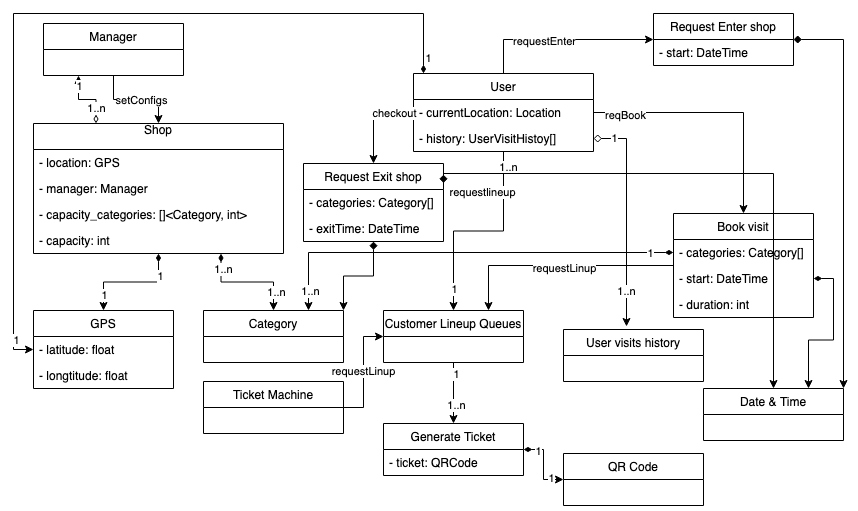
\includegraphics[width=\textwidth,height=\textheight,keepaspectratio]{images/ClassDiagram.png}
  \caption{High level Class Diagram}
  \label{fig:ClassDiagram}
\end{figure}

\subsubsection{State Diagrams}
Now we analyse the some important functions of the application, modelling their behaviours and analyze their behaviour to have the expected functionality. we report these diagrams below. \\

\begin{figure}[H]
  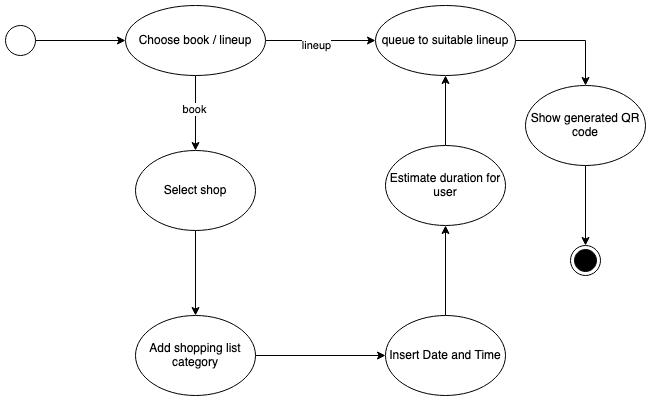
\includegraphics[width=\textwidth,height=\textheight,keepaspectratio]{images/bookLineup.png}
  \caption{User book a visit or insert to lineup queue}
  \label{fig:bookLineup}
\end{figure}

In this (Figure \ref{fig:bookLineup}), we model a user whom has a cell phone and wants to go shopping. As you can see, the user can choose to go to queue or book a visit for a time in future. System could sends him/her list of suggested time and user could choose between them.

\begin{figure}[H]
  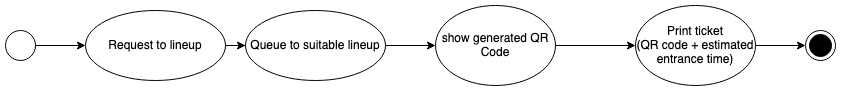
\includegraphics[width=\textwidth,height=\textheight,keepaspectratio]{images/OfflineTicket.png}
  \caption{User get ticket from ticket machine}
  \label{fig:OfflineTicket}
\end{figure}

In this (Figure \ref{fig:OfflineTicket}), we model a user who want to use ticket machine and do not use the app. In this case, user only can add himself/herself to the current line up of the shop.

\begin{figure}[H]
  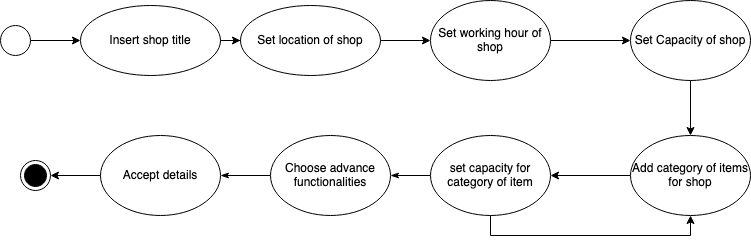
\includegraphics[width=\textwidth,height=\textheight,keepaspectratio]{images/CreateShop.png}
  \caption{Manager create a shop}
  \label{fig:CreateShop}
\end{figure}

In this (Figure \ref{fig:CreateShop}), shows how a manager could create a shop and add necessary information for creating a shop in our system.

\begin{figure}[H]
  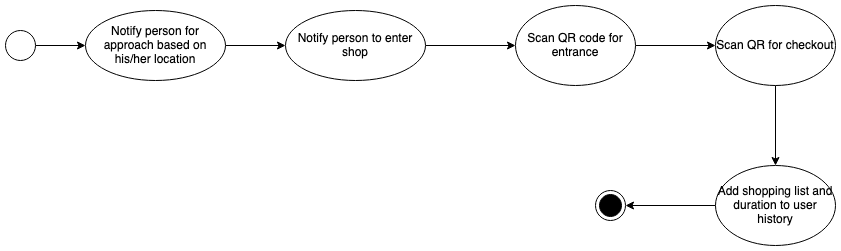
\includegraphics[width=\textwidth,height=\textheight,keepaspectratio]{images/Shopping.png}
  \caption{User shopping}
  \label{fig:shopping}
\end{figure}

In this (Figure \ref{fig:shopping}), we model the behaviour of user from entrance to shop until checkout. In the checkout time, we re-scan the QR code of user to insert data user shopping list and duration to user history. we could use, this information to estimate the behaviour of each user and improve waiting time estimation in our system.

\subsection{Product functions}
1. retrieving a number to line up: the main functionality of the application is the possibility of retrieving a number  which gives them their position in the queue. after then it will be easier for customers to access the supermarket without standing in a line for so long.  this way  forces people to first approach the building and then wait in close proximity (though not in a line) until their number is called.

2. generate QR codes:  this feature would be scanned upon entering the store, thus allowing store managers to monitor entrances.

3. estimation process:  There is a real risk that the approach does not
work in the case the customer arrives to the grocery store after his/her number is called, or too early, as in this case we would get back into a physical line situation. This implies that the system should provide customers with a reasonably precise estimation of the waiting time and should alert them taking into account the time they need to get to the shop from the place they currently are.

4. booking a visit: this function indicate that u can reserve a slot to go to supermarket, its almost like reserving a slot to go to museum or exhibition but they have slight differences like the duration that take to be in a supermarket which we are not able to estimate their time of shopping. so we have to mention a feature which request customer to indicate the approximate expected duration of the visit.

5. system for the customers analysis: there's another option that works for long-term customers in which the time spent by customers is analyzed and the system is gonna predict the average time for that specefic customer based on their pervious visits.

6. indicating the category of items: The application might also allow users to indicate, if not the exact list of items that they intend to
purchase, the categories of items that they intend to buy. This would allow the application to plan visits in a finer way, for example allowing more people in the store, if it knows that they are going to buy different things, hence they will occupy different spaces in the store when they visit (thus respecting the requirement that people keep enough distance between them).

\subsection{User characteristic}
The actors of the application are the following:

\begin{enumerate}
\item \textbf{user:} customers who download this application to go shopping for the groceries but due to Covid-19 stores and supermarkets shouldn't be full of people and they should follow the social distant rule so without application they used to stand in long lines with social distance but with this application which generate QR codes and with other functionalities, we minimize the time spent by each customer in a line by retrieving a number and send them to be in line if their number is getting closer. also they can book a visit from some days before to go for shopping at supermarkets.

\item \textbf{Clerk:} they would scan the QR codes which customers already have by app, and they allow customers to enter. Moreover, stores should also have the possibility to hand out “tickets” on the spot, thus acting as proxies for the customers because maybe some customers do not have the  access to the required technology

\item \textbf{Manager:} the manager is defining the store on our system and he/she assigns the capacity of either the whole store or each section of the that.
\end{enumerate}

\subsection{Assumptions, dependencies and constraints}
Domain assumptions: 
\arrayrulecolor{tableBorderColor}
\setlength\arrayrulewidth{1pt}
\rowcolors{2}{white}{tableHighlightColor}
\setlength\LTleft{0pt}

\begin{longtable}{ !\Vline c !\Vline p{0.9\linewidth} !\Vline}
    \hline
    \textbf{D1} & The internet works properly\\
    \textbf{D2} & Its better for users to have smartphones  \\
    \textbf{D3} & users should be at the spot right on the specific time which is mentioned in the app \\
    \textbf{D4} & the time estimation by the app is correct \\
    \textbf{D5} & Clerks are connected to device Which is registered for the specific shop.\\
     \textbf{D6} & the app is always available and able to generate QR codes\\
    \textbf{D7} & QR code on the ticket of each user must be scan first then let the user to enter the shop.\\
     \textbf{D8} & the QR code shown by users to scanner is valid\\
    \textbf{D9} & At the checkout, QR code on the ticket of each user must be scanned.\\
    \textbf{D10} & the slots shown by app is correct and updated every second for booking part\\
    \textbf{D11} & the QR code generator which called ticket machine for those who doesn't have smartphones works properly all the time\\
    \textbf{D12} & QR code scanner just scan the valid QR codes which means it shouldn't scan after the estimated time.\\
    \textbf{D13} & users do not have much delay at the supermarket and they exit at almost certain time.\\
    \textbf{D14} & Ticket machine should have enough paper to print QR codes for those who doesn't have smartphone.\\
    \textbf{D15} & if users don't have electronic device, they can use QR codes at the supermarket in person by ticket machine.\\
    
    \hline
\end{longtable}

Constraints:
\arrayrulecolor{tableBorderColor}
\setlength\arrayrulewidth{1pt}
\rowcolors{2}{white}{tableHighlightColor}
\setlength\LTleft{0pt}

\begin{longtable}{ !\Vline c !\Vline l !\Vline}
    \hline
    \textbf{C1} & each ticket is valid for entrance from time the system call it turns until 30 minutes later\\
    \hline
\end{longtable}



\section{Specific Requirements}

\subsection{External Interfaces}
\subsubsection{User Interface}
% \subsubsection{UML Description}
The UML below describes at high-level the model of the system to be developed. It considers the basic service together with the advanced function 1 and advanced function 2 previously specified. The UML does not include every class that will be necessary to define the complete architecture of the system.\\
CLup more functions than basic service. The manager registers to the application with all necessary information and the manager could activate the advance function or advance function 2 at any time. The user who use mobile could simply download the application on his/her device and use it and user who doesn't have mobile could easily go near the shop and get a ticket from ticket machine.\\
Here we can identify the main aspect of CLup:
\begin{itemize}
    \item The user could request to be in line for a shop and application shows estimated waiting time to him/her.
    \item The user could book a visit for a shop. This booking contains the date and time user wants to go shopping besides, user can add the categories of item he/she has in shopping list. The application could suggest the user free slots and user book them.
    \item The application based the current location of users must notify them and ask them to approach the shop in a suitable time.
    \item The application must notify people when it's their turn to go shopping.
    \item At the entrance time, the QR code generated in the app must be scanned to ensure they come in the right time.
    \item At the checkout, the cashier must scan the QR code of user and the system must add shopping information (like duration of shopping, category of item which user buy) to user history.
\end{itemize}

\begin{figure}[H]
  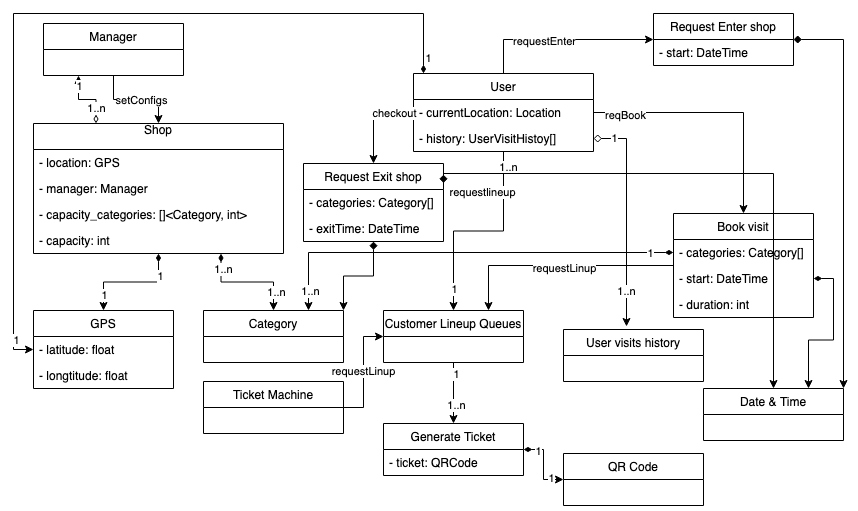
\includegraphics[width=\textwidth,height=\textheight,keepaspectratio]{images/ClassDiagram.png}
  \caption{High level Class Diagram}
  \label{fig:ClassDiagram}
\end{figure}

\subsubsection{State Diagrams}
Now we analyse the some important functions of the application, modelling their behaviours and analyze their behaviour to have the expected functionality. we report these diagrams below. \\

\begin{figure}[H]
  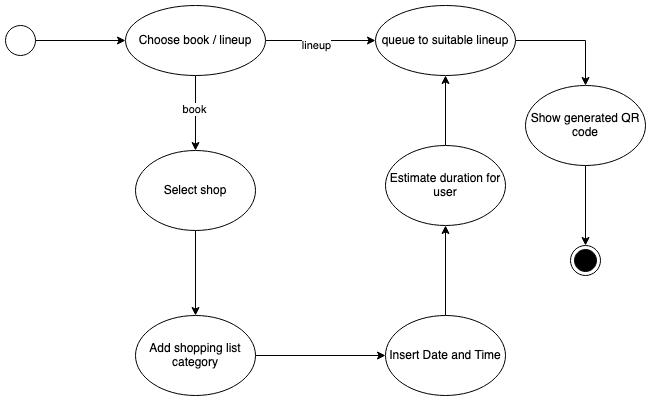
\includegraphics[width=\textwidth,height=\textheight,keepaspectratio]{images/bookLineup.png}
  \caption{User book a visit or insert to lineup queue}
  \label{fig:bookLineup}
\end{figure}

In this (Figure \ref{fig:bookLineup}), we model a user whom has a cell phone and wants to go shopping. As you can see, the user can choose to go to queue or book a visit for a time in future. System could sends him/her list of suggested time and user could choose between them.

\begin{figure}[H]
  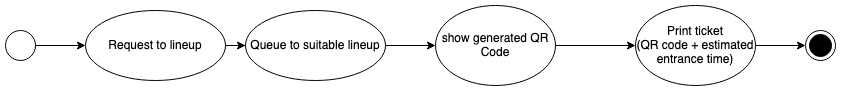
\includegraphics[width=\textwidth,height=\textheight,keepaspectratio]{images/OfflineTicket.png}
  \caption{User get ticket from ticket machine}
  \label{fig:OfflineTicket}
\end{figure}

In this (Figure \ref{fig:OfflineTicket}), we model a user who want to use ticket machine and do not use the app. In this case, user only can add himself/herself to the current line up of the shop.

\begin{figure}[H]
  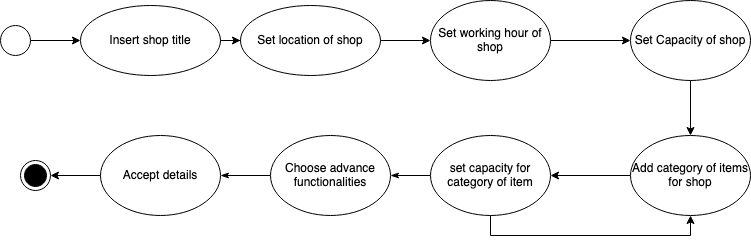
\includegraphics[width=\textwidth,height=\textheight,keepaspectratio]{images/CreateShop.png}
  \caption{Manager create a shop}
  \label{fig:CreateShop}
\end{figure}

In this (Figure \ref{fig:CreateShop}), shows how a manager could create a shop and add necessary information for creating a shop in our system.

\begin{figure}[H]
  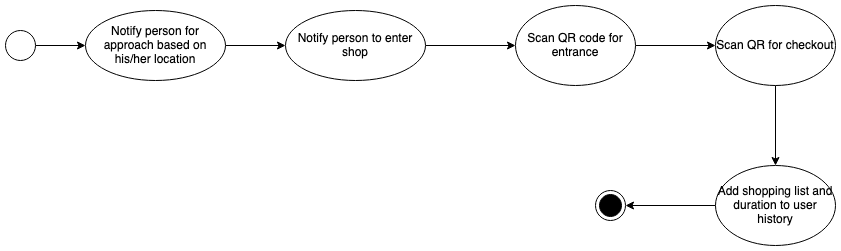
\includegraphics[width=\textwidth,height=\textheight,keepaspectratio]{images/Shopping.png}
  \caption{User shopping}
  \label{fig:shopping}
\end{figure}

In this (Figure \ref{fig:shopping}), we model the behaviour of user from entrance to shop until checkout. In the checkout time, we re-scan the QR code of user to insert data user shopping list and duration to user history. we could use, this information to estimate the behaviour of each user and improve waiting time estimation in our system.
The application that we are using should be able to generate QR codes and will appear in the screen for customers to use. before that, we assume that users already inserted the specific shop they want to go and also choose between two mode of lining up and book a visit for that supermarket later. the app show  estimated time and the number of people before that user so they can save their time and  mange their life better. after all they will scan their QR code and enter the supermarket.
A smartphone and within that, the application, is the suitable thing that answer the needs.
the following mockups give the idea of:
1. The logo of the application looks like;
2. The splash screens;
3. And the 4 first pages of the application;
\begin{figure}[H]
  \centering
  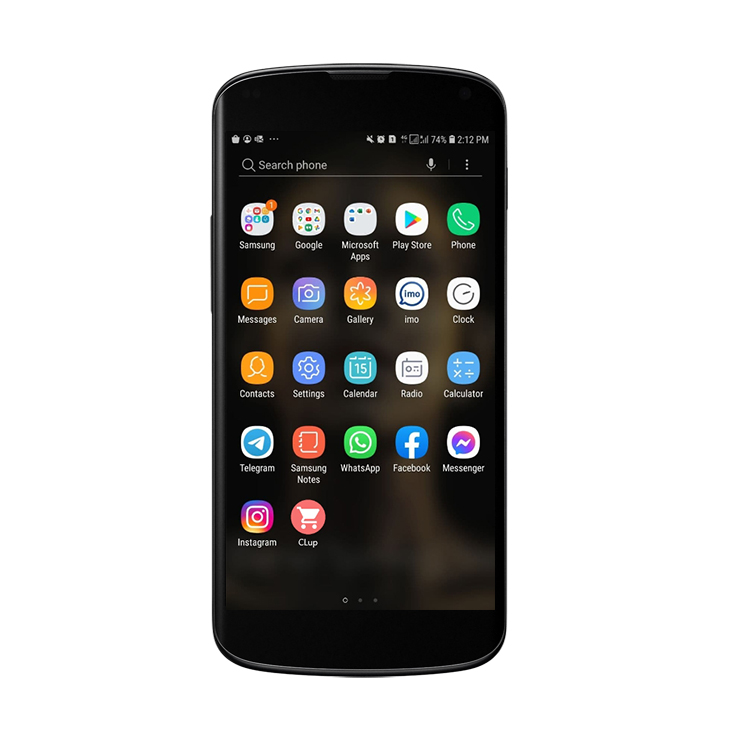
\includegraphics[width=0.7\textwidth,keepaspectratio]{images/1.jpg}
  \caption{Icon Mockup}
\end{figure}
\begin{figure}[H]
  \centering
  
\includegraphics[width=0.7\textwidth,keepaspectratio]{images/2.png}
  \caption{Openning page Mockup}
\end{figure}
\begin{figure}[H]
  \centering
  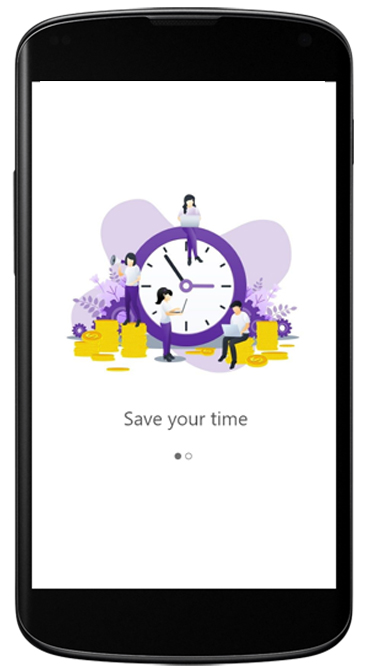
\includegraphics[width=0.7\textwidth,keepaspectratio]{images/3.jpg}
  \caption{Splash Screen Mockup}
\end{figure}
\begin{figure}[H]
  \centering
  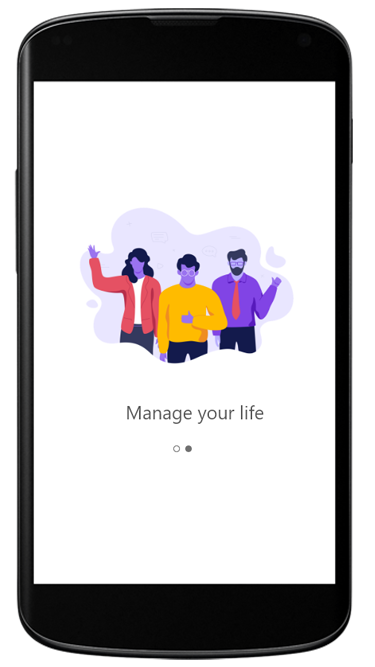
\includegraphics[width=0.7\textwidth,keepaspectratio]{images/4.png}
  \caption{Splash Screen Mockup}
\end{figure}
\begin{figure}[H]
  \centering
  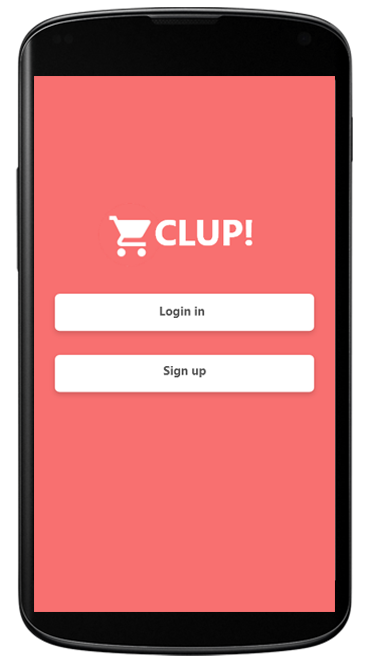
\includegraphics[width=0.7\textwidth,keepaspectratio]{images/5.png}
  \caption{Sign up/log in page Mockup}
\end{figure}
\begin{figure}[H]
  \centering
  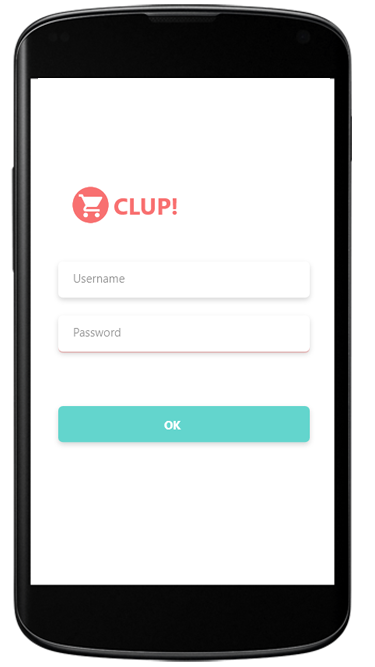
\includegraphics[width=0.7\textwidth,keepaspectratio]{images/6.png}
  \caption{Log in Mockup}
\end{figure}
\begin{figure}[H]
  \centering
  
\includegraphics[width=0.7\textwidth,keepaspectratio]{images/7.png}
  \caption{Sign up Mockup}
\end{figure}
\begin{figure}[H]
  \centering
  
\includegraphics[width=0.7\textwidth,keepaspectratio]{images/8.png}
  \caption{Sign up (II) Mockup}
\end{figure}
\begin{figure}[H]
  \centering
  
\includegraphics[width=0.7\textwidth,keepaspectratio]{images/9.png}
  \caption{home page Mockup}
\end{figure}
\begin{figure}[H]
  \centering
  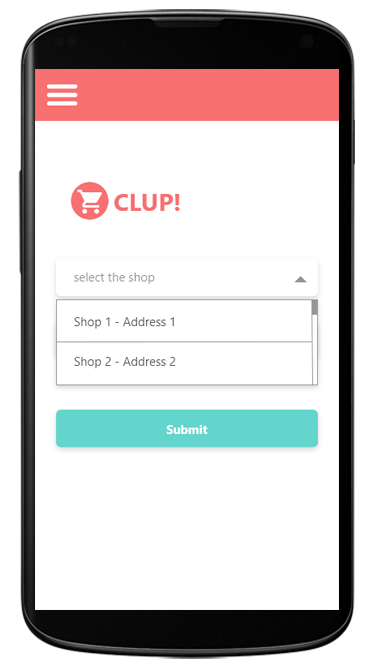
\includegraphics[width=0.7\textwidth,keepaspectratio]{images/10.png}
  \caption{home page (II) Mockup}
\end{figure}
\begin{figure}[H]
  \centering
  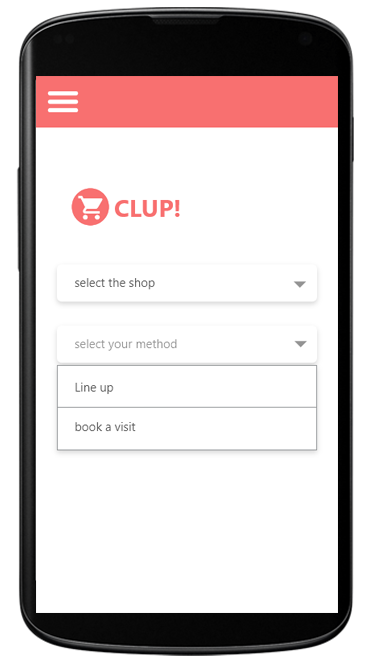
\includegraphics[width=0.7\textwidth,keepaspectratio]{images/11.png}
  \caption{home page (III) Mockup}
\end{figure}
other mockups will be presented in the Design Document part for User Interfaces.

\subsection{Functional Requirements}
\setcounter{tocdepth}{4}
\setcounter{secnumdepth}{4}

\subsubsection{List of requirements}

\arrayrulecolor{tableBorderColor}
\setlength\arrayrulewidth{1pt}
\rowcolors{2}{white}{tableHighlightColor}
\setlength\LTleft{0pt}

\begin{longtable}{ !\Vline c !\Vline p{0.9\linewidth} !\Vline}
    \hline
    \textbf{R1} & Users certified with an authentication\\
    \textbf{R2} & Managers certified with an authentication\\
    \textbf{R3} & Managers should register to the application by a form with mandatory fields\\
    \textbf{R4} & Only managers can create shop\\
    \textbf{R5} & Only managers can update their shop\\
    \textbf{R6} & Managers can activate advance function 1 (allow users booking) on their shop\\
    \textbf{R7} & Managers can activate advance function 2 (send suggestions) on their shop\\
    \textbf{R8} & Users must accept the GPS location for the application\\
    \textbf{R9} & Users could see the list of shops are around them\\
    \textbf{R10} & Users could go to current line-up queue for specific shop \\
    \textbf{R11} & Users could see their ticket (QR code) and estimated waiting time \\
    \textbf{R12} & Users could choose book a time to visit specific shop \\
    \textbf{R13} & Users could choose for which categories they go shopping when they book a visit \\
    \textbf{R14} & The system must generate suitable QR code\\
    \textbf{R15} & The system must estimate the waiting time for each user\\
    \textbf{R16} & The system must make current line-up queue based on users booking\\
    \textbf{R17} & The system sends a notification to user to approach shop based on current location of user and location of shop\\
    \textbf{R18} & The system sends a notification to user to go to the shop when it's him/her turn\\
    \textbf{R19} & After user ticket scanned for entrance, system change status of ticket to invalidate for entrance\\
    \textbf{R20} & The clerk must scan the user ticket\\
    \textbf{R21} & The clerk could add a person to current line-up queue\\
    \textbf{R22} & The clerk could print ticket\\
    \textbf{R23} & After the user checked out, the system analyze shopping list and duration time and add it to the user's visit history \\
    \textbf{R24} & The system could estimate the category of shopping and duration of shopping for specific user \\
    \textbf{R25} & The system estimate the time based on user characteristic\\
    \textbf{R26} & Users can ask a clerk to give them a ticket\\
    \textbf{R27} & If specific time past from user turn to enter his/her ticket will be invalidate for entrance\\
    \textbf{R28} & If managers update a shop the estimated time and book visits will be recalculate\\
    \textbf{R29} & Manager choose the capacity of shop\\
    \textbf{R30} & Manager choose the category of each section in the shop and their capacity\\
    \textbf{R31} & Manager choose working hour of the shop\\
    \hline
\end{longtable}

\subsubsection{Mapping}

\subsubsection{Use cases}
\paragraph{Use case Description} \hfill
\begin{itemize}

\item \textbf{Register}
\arrayrulecolor{tableBorderColor}
\setlength\arrayrulewidth{1pt}
\rowcolors{2}{white}{tableHighlightColor}
\setlength\LTleft{0pt}
\begin{longtable}{ !\Vline c !\Vline p{0.9\linewidth} !\Vline}
    \hline
    \textbf{Name} & \textbf{Register}\\
    \textbf{ID} & UC1\\
    \textbf{Actors} & Super User\\
    \textbf{Entry Condition} & Super User has internet connection on his/her device\\
    \textbf{Event flow} & 
    \begin{enumerate}
        \item Super user see the landing page
        \item Super user click on the "sign up" button
        \item Super user fill all the mandatory fields
        \item Super user choose his type between manager or user
        \item Super user fill extra fields based on his type
        \item Super user click on "Register" button
        \item The system validate the filled data
        \item The system confirm the registration
        \item The system save the super user on database
    \end{enumerate}\\
    \textbf{Exit Condition} & Super user is successfully registered in the system\\
    \textbf{Exceptions} & 
    If the below conditions happened the application return a suitable error in message and return to register page.
    \begin{itemize}
        \item Super user is already existed in the system
        \item Super user doesn't fill all mandatory fields
        \item Super user sends invalid data
    \end{itemize}
    
    \\
    \hline
\end{longtable}

\item \textbf{Login}
\arrayrulecolor{tableBorderColor}
\setlength\arrayrulewidth{1pt}
\rowcolors{2}{white}{tableHighlightColor}
\setlength\LTleft{0pt}
\begin{longtable}{ !\Vline c !\Vline p{0.9\linewidth} !\Vline}
    \hline
    \textbf{Name} & \textbf{Login}\\
    \textbf{ID} & UC2\\
    \textbf{Actors} & Super User\\
    \textbf{Entry Condition} & Super User has internet connection and it already registered to the application\\
    \textbf{Event flow} & 
    \begin{enumerate}
        \item Super user see the landing page
        \item Super user click on the "sign in" button
        \item Super user fill username and password fields
        \item Super user click on "Login" button
        \item The system check the credential
        \item The system confirm the registration
        \item The system return the home page of user
    \end{enumerate}\\
    \textbf{Exit Condition} & Super user has access to the service of CLup\\
    \textbf{Exceptions} & 
    If the below conditions happened the application return a suitable error in message and return to login page.
    \begin{itemize}
        \item Super user is not exist in the system
        \item Super user doesn't fill all mandatory fields
        \item Super user password is invalid
    \end{itemize}
    
    \\
    \hline
\end{longtable}

\item \textbf{Create shop}
\arrayrulecolor{tableBorderColor}
\setlength\arrayrulewidth{1pt}
\rowcolors{2}{white}{tableHighlightColor}
\setlength\LTleft{0pt}
\begin{longtable}{ !\Vline c !\Vline p{0.9\linewidth} !\Vline}
    \hline
    \textbf{Name} & \textbf{Create Shop}\\
    \textbf{ID} & UC3\\
    \textbf{Actors} & Manager\\
    \textbf{Entry Condition} & Manager has internet connection\\
    \textbf{Event flow} & 
    \begin{enumerate}
        \item Manager see the home page
        \item Manager click on the "add a shop" button
        \item Manager set shop title
        \item Manager set location of the shop
        \item Manager set start and end hour of the shop
        \item Manager set capacity of the shop
        \item manager click on "new category"
        \item manager set capacity and title of category
        \item click on "end" button or return to 7.
        \item manager choose AF1 or AF2 enable by checkbox.
        \item manager click on "Submit" button.
        \item The system shows all the detail of shop.
        \item manager click on "Accept" button.
        \item The system add shop to data base.
    \end{enumerate}\\
    \textbf{Exit Condition} & Shop successfully created\\
    \textbf{Exceptions} & If the data of shop is not valid the sytem will return error\\
    \hline
\end{longtable}

\item \textbf{Update shop}
\arrayrulecolor{tableBorderColor}
\setlength\arrayrulewidth{1pt}
\rowcolors{2}{white}{tableHighlightColor}
\setlength\LTleft{0pt}
\begin{longtable}{ !\Vline c !\Vline p{0.9\linewidth} !\Vline}
    \hline
    \textbf{Name} & \textbf{Create Shop}\\
    \textbf{ID} & UC4\\
    \textbf{Actors} & Manager\\
    \textbf{Entry Condition} & Manager has internet connection and the shop is exists\\
    \textbf{Event flow} & 
    \begin{enumerate}
        \item Manager see the home page
        \item Manager click on the "edit" button in specific shop
        \item Manager change fields it like
        \item manager click on "Submit" button.
        \item The system shows all the detail of shop.
        \item manager click on "Accept" button.
        \item The system update the shop in data base.
        \item The system update recalculate the estimated time by new values.
    \end{enumerate}\\
    \textbf{Exit Condition} & Shop successfully updated\\
    \textbf{Exceptions} & 
        If the below conditions happened the application return a suitable error.
    \begin{itemize}
        \item Shop is not existed in the system.
        \item Manager doesn't have access to change that shop.
        \item Fields values are invalid.
    \end{itemize}\\
    \hline
\end{longtable}

\item \textbf{See list of shops}
\arrayrulecolor{tableBorderColor}
\setlength\arrayrulewidth{1pt}
\rowcolors{2}{white}{tableHighlightColor}
\setlength\LTleft{0pt}
\begin{longtable}{ !\Vline c !\Vline p{0.9\linewidth} !\Vline}
    \hline
    \textbf{Name} & \textbf{See list of shops}\\
    \textbf{ID} & UC5\\
    \textbf{Actors} & User\\
    \textbf{Entry Condition} & User has internet connection and must accept GPS permission\\
    \textbf{Event flow} & 
    \begin{enumerate}
        \item User get latitude and longitude from GPS
        \item User send a request to get list of shops
        \item The system extract latitude and longitude from user request
        \item The system get shop list from database
        \item The system order shops based on latitude and longitude and characteristic of user.
        \item The system shows the list of shops to user.
    \end{enumerate}\\
    \textbf{Exit Condition} & User see list of shops\\
    \textbf{Exceptions} & None\\
    \hline
\end{longtable}


\item \textbf{Generate ticket}
\arrayrulecolor{tableBorderColor}
\setlength\arrayrulewidth{1pt}
\rowcolors{2}{white}{tableHighlightColor}
\setlength\LTleft{0pt}
\begin{longtable}{ !\Vline c !\Vline p{0.9\linewidth} !\Vline}
    \hline
    \textbf{Name} & \textbf{Generate ticket}\\
    \textbf{ID} & UC6\\
    \textbf{Actors} & User, Clerk\\
    \textbf{Entry Condition} & user or clerk wants to add to a line-up queue\\
    \textbf{Event flow} & 
    \begin{enumerate}
        \item The system extract the user turn.
        \item The system extract the user id.
        \item The system extract the shop id.
        \item The system extract the line-up queue id.
        \item The system generate a QR code based on those information.
        \item The system saves generated QR code to database.
        \item The system shows the generated QR code to user.
    \end{enumerate}\\
    \textbf{Exit Condition} & QR code generated successfully \\
    \textbf{Exceptions} & None\\
    \hline
\end{longtable}

\item \textbf{Estimate waiting time}
\arrayrulecolor{tableBorderColor}
\setlength\arrayrulewidth{1pt}
\rowcolors{2}{white}{tableHighlightColor}
\setlength\LTleft{0pt}
\begin{longtable}{ !\Vline c !\Vline p{0.9\linewidth} !\Vline}
    \hline
    \textbf{Name} & \textbf{Estimate waiting time}\\
    \textbf{ID} & UC7\\
    \textbf{Actors} & User, Clerk\\
    \textbf{Entry Condition} & user or clerk wants to add to a line-up queue\\
    \textbf{Event flow} & 
    \begin{enumerate}
        \item The system extract the users from line-up queue.
        \item The system extract the shop.
        \item The system extract the new user wants to add in line up.
        \item The system get history of users shopping from database.
        \item The system extract new user wants shop from which categories.
        \item based on previous behavior of user and categories system estimate shopping duration of user.
        \item based on previous users in queue, system estimate waiting time for user.
    \end{enumerate}\\
    \textbf{Exit Condition} & The system estimate the user waiting time \\
    \textbf{Exceptions} & Check the shops, users and line-up queue are really exists. if they are not exist send a proper message.\\
    \hline
\end{longtable}

\item \textbf{Add to Line-up Queue}
\arrayrulecolor{tableBorderColor}
\setlength\arrayrulewidth{1pt}
\rowcolors{2}{white}{tableHighlightColor}
\setlength\LTleft{0pt}
\begin{longtable}{ !\Vline c !\Vline p{0.9\linewidth} !\Vline}
    \hline
    \textbf{Name} & \textbf{Add to Line-up Queue}\\
    \textbf{ID} & UC8\\
    \textbf{Actors} & User, Clerk\\
    \textbf{Entry Condition} & user choose specific shop to go to one of it lines up queue or user book a visit, clerk wants to add person do not use application to a line-up queue\\
    \textbf{Event flow} & 
    \begin{enumerate}
        \item User choose a shop to add line up or book a visit for that shop or clerk click on add to line-up.
        \item The system find that line-up queue
        \item The system get the generate number of user in queue.
        \item The system pass user, shop and queue to [UC6].
        \item The system get the QR code of ticket.
        \item The system pass user, shop and queue to [UC7].
        \item The system get the estimation waiting time for user.
        \item The system get current location of user.
        \item The system get calculate traveling time estimation for user.
        \item The system set interval to send notification for approach a user.
        \item The system add user to correct line-up queue.
        \item The system send ticket and estimated time to user.
    \end{enumerate}\\
    \textbf{Exit Condition} & add user to line-up queue \\
    \textbf{Exceptions} & None\\
    \hline
\end{longtable}

\item \textbf{Book a visit}
\arrayrulecolor{tableBorderColor}
\setlength\arrayrulewidth{1pt}
\rowcolors{2}{white}{tableHighlightColor}
\setlength\LTleft{0pt}
\begin{longtable}{ !\Vline c !\Vline p{0.9\linewidth} !\Vline}
    \hline
    \textbf{Name} & \textbf{Book a visit}\\
    \textbf{ID} & UC9\\
    \textbf{Actors} & User\\
    \textbf{Entry Condition} & The shop AF1 is activate and user choose book\\
    \textbf{Event flow} & 
    \begin{enumerate}
        \item User choose a shop.
        \item User click on "book a visit" button.
        \item The user choose date and time.
        \item The system returns items' category of that shop.
        \item User add category of items wants to buy.
        \item Based on date user choose system finds a suitable queue.
        \item Pass the parameters to [UC8] and get the result.
        \item Get the ticket and show it.
    \end{enumerate}\\
    \textbf{Exit Condition} & user successfully book a visit \\
    \textbf{Exceptions} & If user the queue capacity is full\\
    \hline
\end{longtable}

\item \textbf{See ticket}
\arrayrulecolor{tableBorderColor}
\setlength\arrayrulewidth{1pt}
\rowcolors{2}{white}{tableHighlightColor}
\setlength\LTleft{0pt}
\begin{longtable}{ !\Vline c !\Vline p{0.9\linewidth} !\Vline}
    \hline
    \textbf{Name} & \textbf{See ticket}\\
    \textbf{ID} & UC10\\
    \textbf{Actors} & User\\
    \textbf{Entry Condition} & The user has a ticket for that shop\\
    \textbf{Event flow} & 
    \begin{enumerate}
        \item User choose a shop.
        \item User click on "ticket" button.
        \item The system find the ticket.
        \item The system calculate remaining time.
        \item The system return the QR code and estimation time.
    \end{enumerate}\\
    \textbf{Exit Condition} & user get the ticket \\
    \textbf{Exceptions} & If user is doesn't have the ticket for that shop system return a message\\
    \hline
\end{longtable}

\item \textbf{Notify user for approach}
\arrayrulecolor{tableBorderColor}
\setlength\arrayrulewidth{1pt}
\rowcolors{2}{white}{tableHighlightColor}
\setlength\LTleft{0pt}
\begin{longtable}{ !\Vline c !\Vline p{0.9\linewidth} !\Vline}
    \hline
    \textbf{Name} & \textbf{Notify user for approach}\\
    \textbf{ID} & UC11\\
    \textbf{Actors} & Time\\
    \textbf{Entry Condition} & Timer that [UC8] set, finished\\
    \textbf{Event flow} & 
    \begin{enumerate}
        \item The system sends a request to notification system.
        \item The notification system send a notification to user.
    \end{enumerate}\\
    \textbf{Exit Condition} & user get notification \\
    \textbf{Exceptions} & none\\
    \hline
\end{longtable}

\item \textbf{Print ticket}
\arrayrulecolor{tableBorderColor}
\setlength\arrayrulewidth{1pt}
\rowcolors{2}{white}{tableHighlightColor}
\setlength\LTleft{0pt}
\begin{longtable}{ !\Vline c !\Vline p{0.9\linewidth} !\Vline}
    \hline
    \textbf{Name} & \textbf{Print ticket}\\
    \textbf{ID} & UC13\\
    \textbf{Actors} & Clerk\\
    \textbf{Entry Condition} & A person doesn't use mobile ask clerk for a ticket\\
    \textbf{Event flow} & 
    \begin{enumerate}
        \item The clerk click "ticket" on ticket machine.
        \item The system add an anonymous user to queue by [UC9].
        \item The system show ticket.
        \item The clerk click on "print" button.
        \item The printer print the ticket.
    \end{enumerate}\\
    \textbf{Exit Condition} & anonymous user got to queue and ticket printed\\
    \textbf{Exceptions} & none\\
    \hline
\end{longtable}

\item \textbf{Scan QR code for entrance}
\arrayrulecolor{tableBorderColor}
\setlength\arrayrulewidth{1pt}
\rowcolors{2}{white}{tableHighlightColor}
\setlength\LTleft{0pt}
\begin{longtable}{ !\Vline c !\Vline p{0.9\linewidth} !\Vline}
    \hline
    \textbf{Name} & \textbf{Scan QR code for entrance}\\
    \textbf{ID} & UC14\\
    \textbf{Actors} & Clerk\\
    \textbf{Entry Condition} & A person want to enter the shop\\
    \textbf{Event flow} & 
    \begin{enumerate}
        \item The person show his/her ticket on mobile or printed ticket.
        \item The clerk scan QR code.
        \item The system check can the user enter.
        \item The system remove user from line-up queue.
        \item The system change ticket status invalid for entrance.
        \item The system set start time for user.
    \end{enumerate}\\
    \textbf{Exit Condition} & user can enter the shop\\
    \textbf{Exceptions} & If it isn't user turn red flash light blink on scanner\\
    \hline
\end{longtable}

\item \textbf{checkout}
\arrayrulecolor{tableBorderColor}
\setlength\arrayrulewidth{1pt}
\rowcolors{2}{white}{tableHighlightColor}
\setlength\LTleft{0pt}
\begin{longtable}{ !\Vline c !\Vline p{0.9\linewidth} !\Vline}
    \hline
    \textbf{Name} & \textbf{checkout}\\
    \textbf{ID} & UC15\\
    \textbf{Actors} & Clerk\\
    \textbf{Entry Condition} & A person want to checkout the shop\\
    \textbf{Event flow} & 
    \begin{enumerate}
        \item The person show his/her ticket on mobile or printed ticket.
        \item The clerk scan QR code.
        \item The system find the user.
        \item The clerk scan bar code of items with his/her scanner.
        \item The system find category of items and add to user history.
        \item The system set end time for user and calculate the duration.
        \item The system add user history to database.
        \item The system call the next person turn.
        \item The system set a 1 minute timer to notify next person.
    \end{enumerate}\\
    \textbf{Exit Condition} & user checkout and exit the shop\\
    \textbf{Exceptions} & If user lost his ticket act him as an anonymous user.\\
    \hline
\end{longtable}

\item \textbf{checkout}
\arrayrulecolor{tableBorderColor}
\setlength\arrayrulewidth{1pt}
\rowcolors{2}{white}{tableHighlightColor}
\setlength\LTleft{0pt}
\begin{longtable}{ !\Vline c !\Vline p{0.9\linewidth} !\Vline}
    \hline
    \textbf{Name} & \textbf{checkout}\\
    \textbf{ID} & UC16\\
    \textbf{Actors} & Time\\
    \textbf{Entry Condition} & Timer that [UC15] set finished.\\
    \textbf{Event flow} & 
    \begin{enumerate}
        \item The system change ticket of user to valid.
        \item The system sends a request to notification system.
        \item The notification system send a notification to user.
    \end{enumerate}\\
    \textbf{Exit Condition} & user get notification\\
    \textbf{Exceptions} & None\\
    \hline
\end{longtable}

\end{itemize}

\paragraph{Use case Diagram}

\begin{figure}[H]
  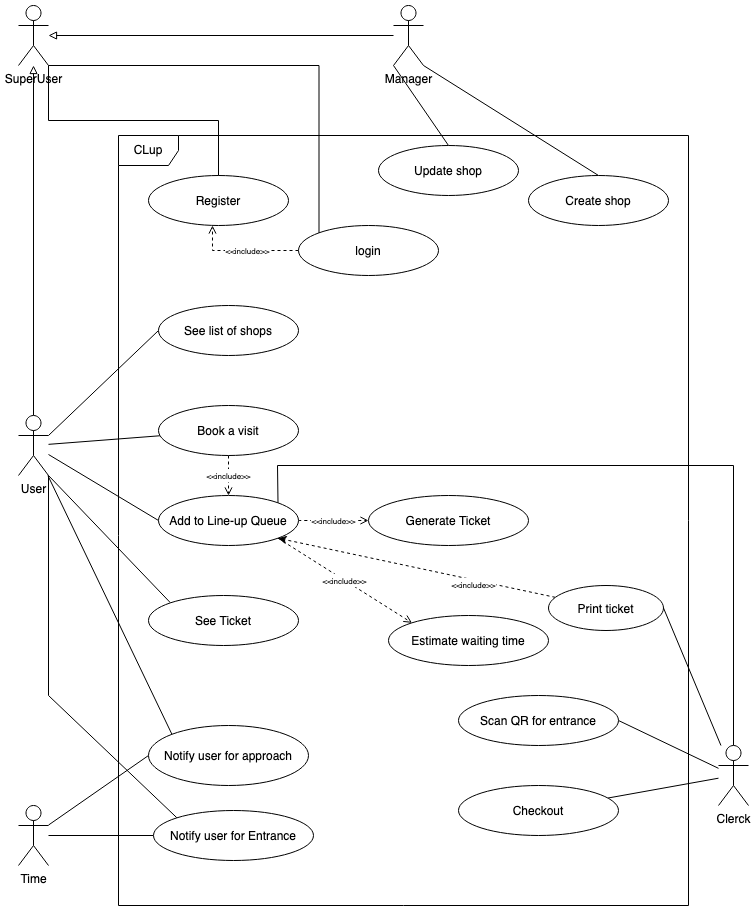
\includegraphics[width=\textwidth,height=\textheight,keepaspectratio]{images/Usecase.png}
  \caption{Use case diagram}
  \label{fig:usecase}
\end{figure}


\setcounter{tocdepth}{3}
\setcounter{secnumdepth}{3}




\section{Formal Analysis Using Alloy}

%%
% Alloy language definition for using with the listings package.
%
% 2017, Daniel Andrade
% BSD 3-Clause License
%%
\definecolor{codegreen}{rgb}{0,0.6,0}
\definecolor{codeblue}{rgb}{0,0.0,0.6}
\lstdefinelanguage{alloy}{
	morekeywords={
		module, open, as,
		private, abstract, sig, extends, in,
		lone, some, one, disj,
		fact, pred, fun, assert,
		run, check,
		for, but, exactly,
		this, not, implies, else, let,
		not, no, set, all, sum,
		iff, or, Int, and,
		none, univ, iden
	},
	sensitive=true,
	morecomment=[l]{//},
	morecomment=[l]{--},
	morecomment=[s]{/*}{*/},
	morestring=[b]{"},
	commentstyle=\color{codegreen},
	keywordstyle=\bf \color{codeblue},
	%literate={->}{$\rightarrow$}1
	% replacing characters can cause problems when copying from PDF to editor
}[keywords,comments,strings]

% define a style for the alloy language
\lstdefinestyle{alloy}{
	commentstyle=\itshape,
	keywordstyle=\bfseries,
	stringstyle=\itshape,
}

% define command for inline use; usage: \alloy|sig A {f: some B}|
\def\alloy{\lstinline[
	language=alloy,
	style=alloy,
	basicstyle=\ttfamily\small
]}

\renewcommand{\ttdefault}{pcr}  % font type with bfseries and ttfamily
% general definitions
\lstset{
	basicstyle=\ttfamily\large
}

\subsection{Alloy Code}
\lstinputlisting[language=alloy,breaklines=true]{parts/section4/alloy.als}
\clearpage

\subsection{Meta Model}

\begin{figure}[H]
	\centering
	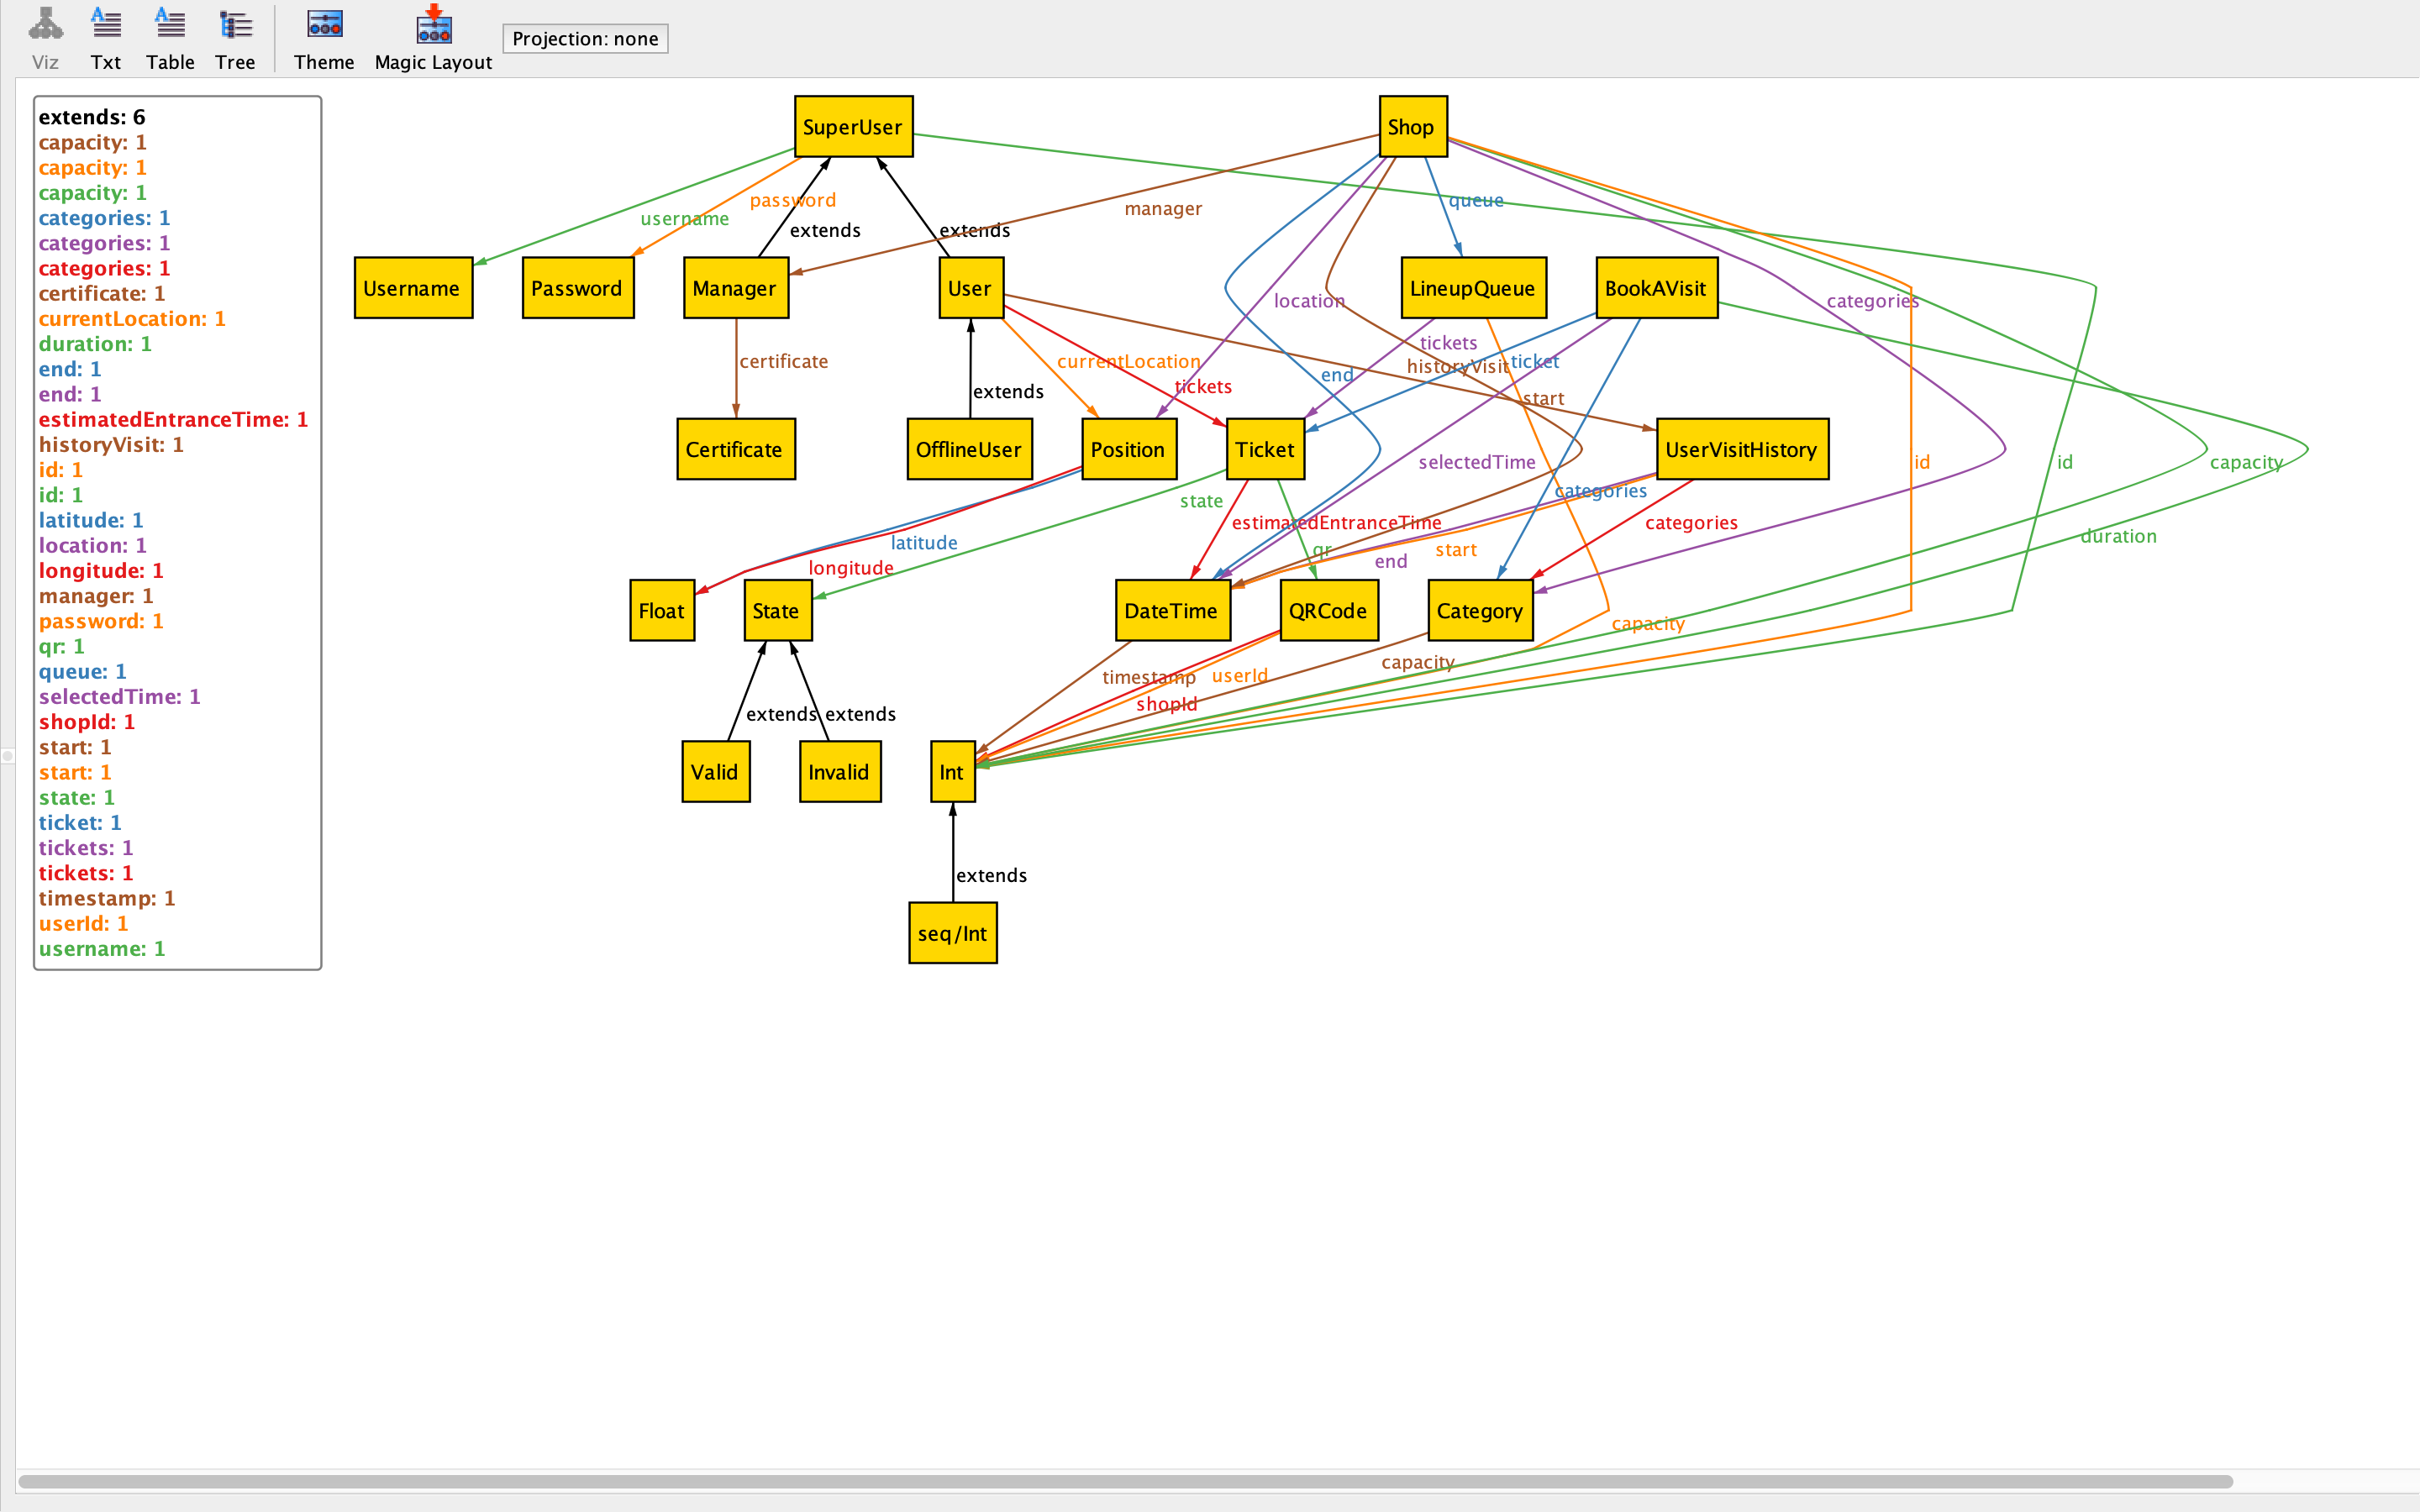
\includegraphics[width=0.9\textheight,keepaspectratio, angle=90]{images/alloy_metamodel.png}
	\caption{Meta model}
\end{figure}
\clearpage

\subsection{Predictions Result}
\begin{enumerate}
	\item Create shop \\
	\begin{figure}[H]
		\centering
		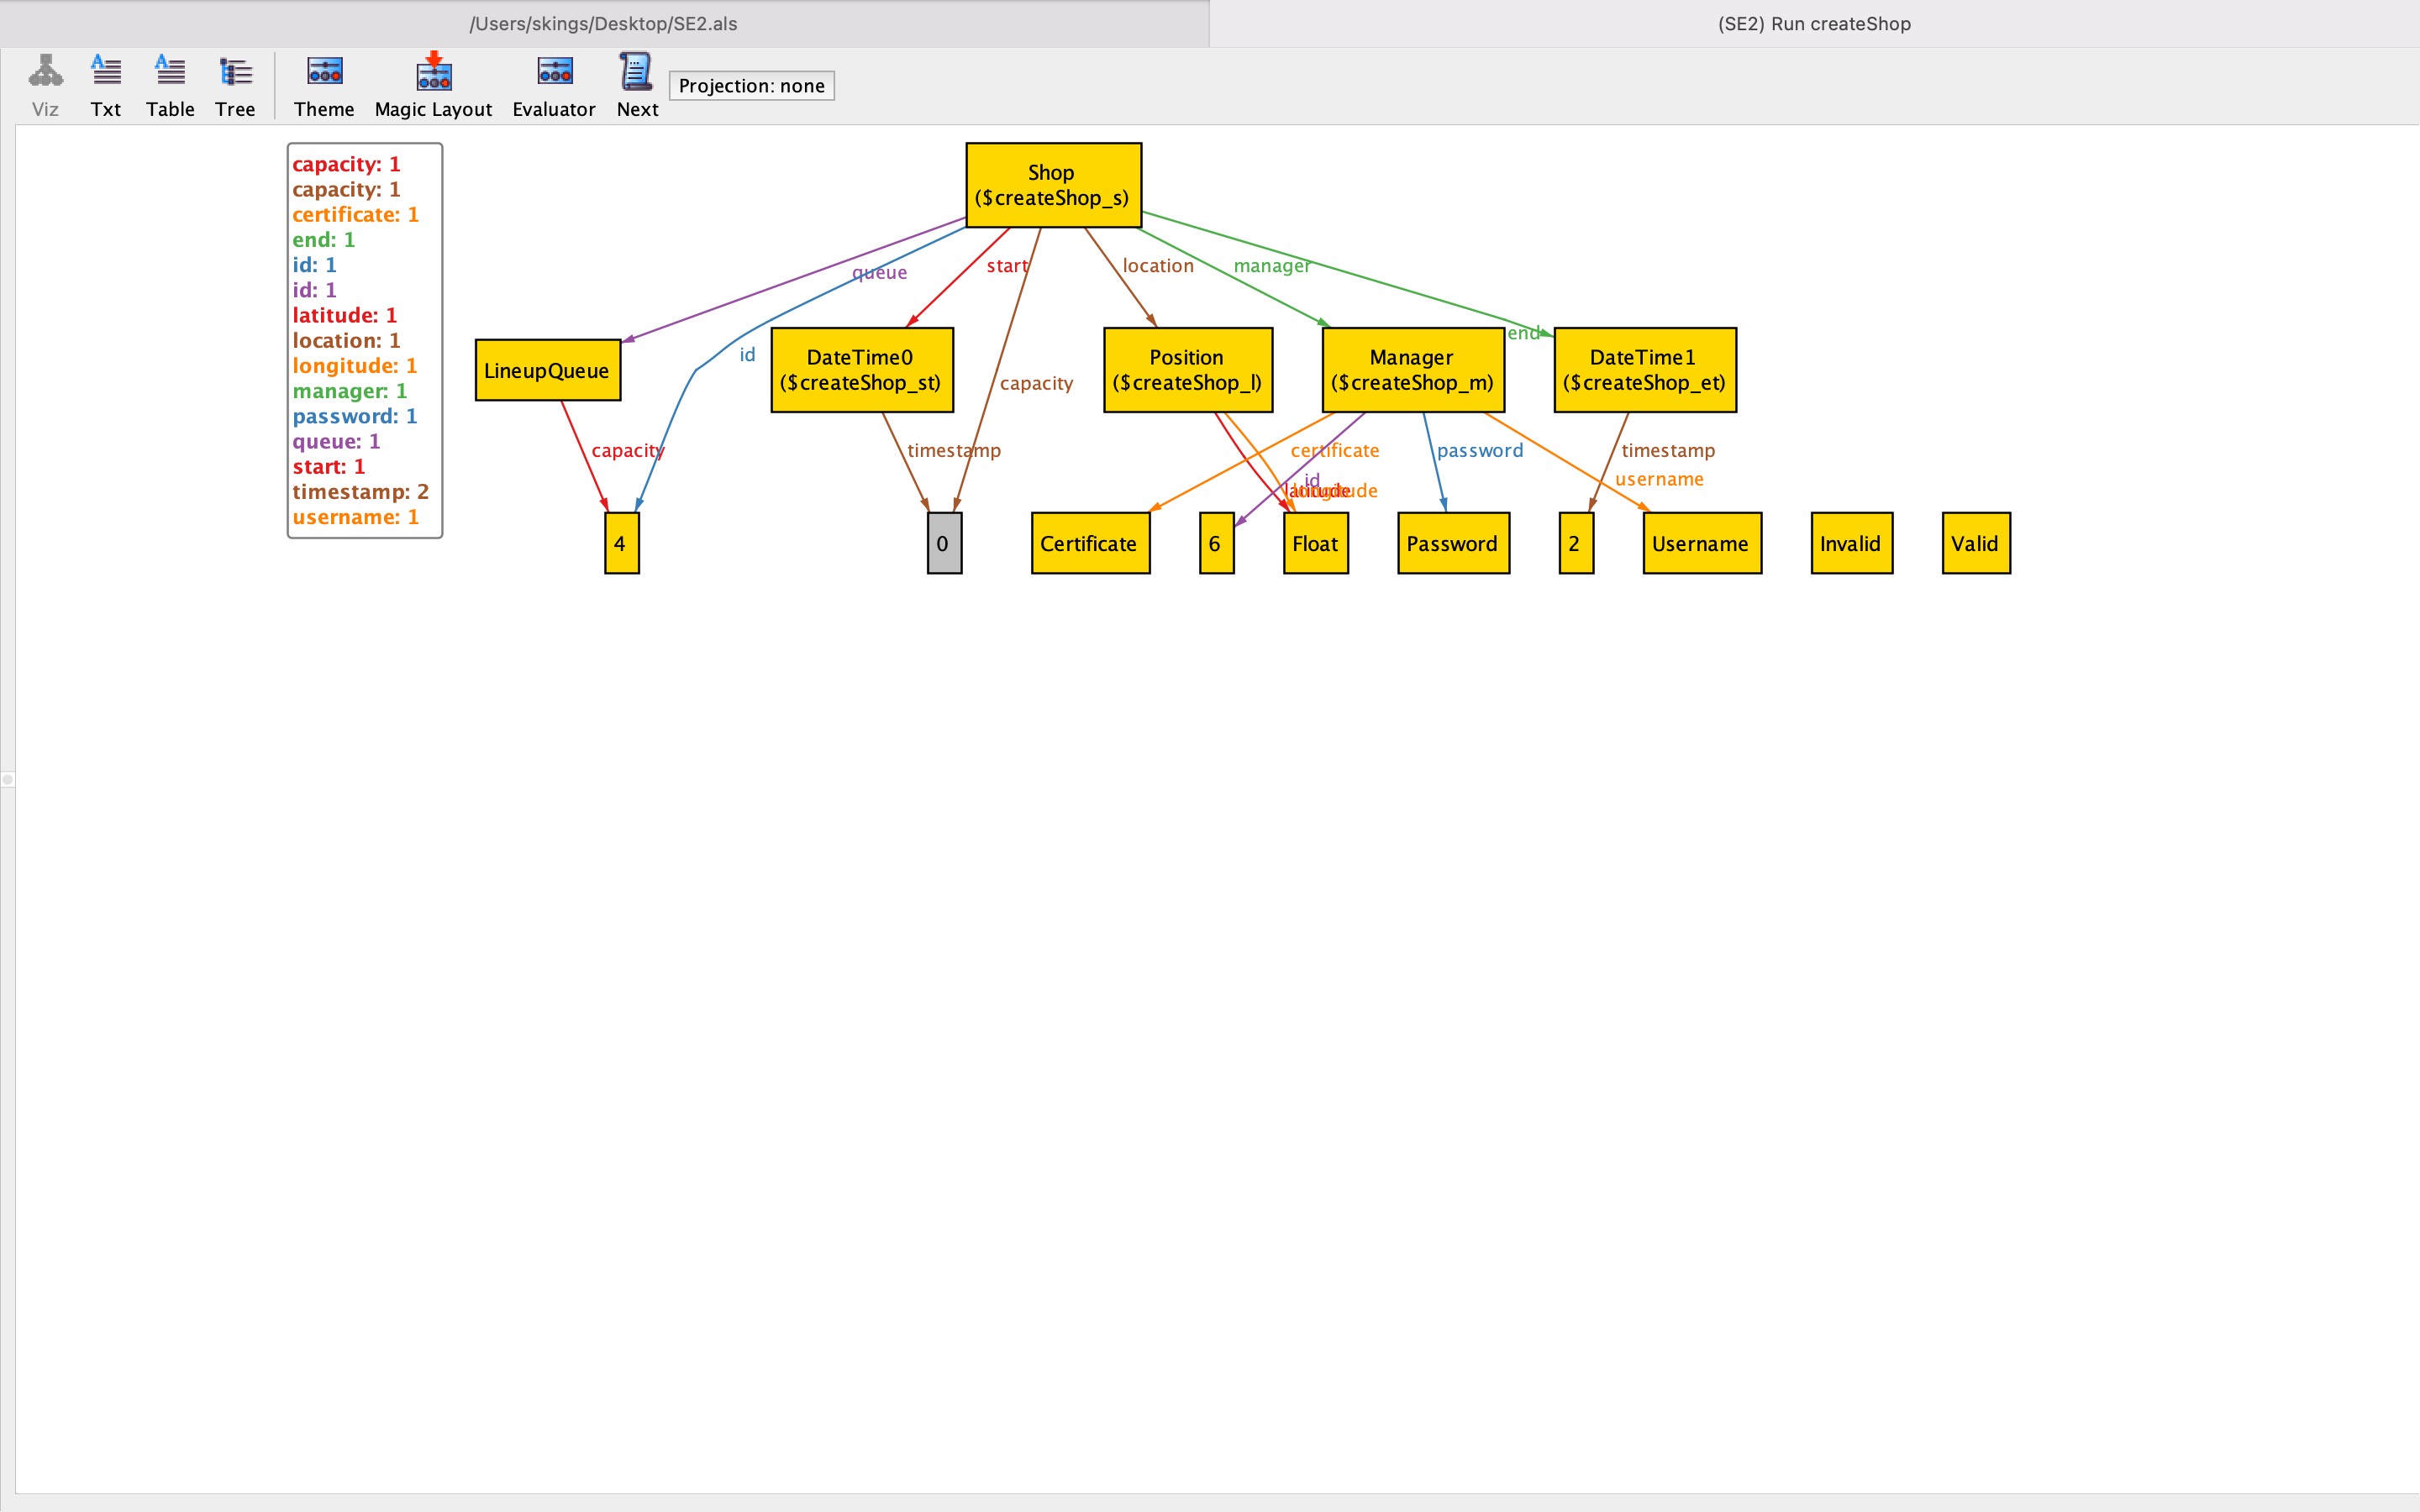
\includegraphics[width=0.9\textheight,keepaspectratio, angle=90]{images/alloy_createShop.png}
	\end{figure}
	\clearpage

	\item Add to line-up \\
	\begin{figure}[H]
		\centering
		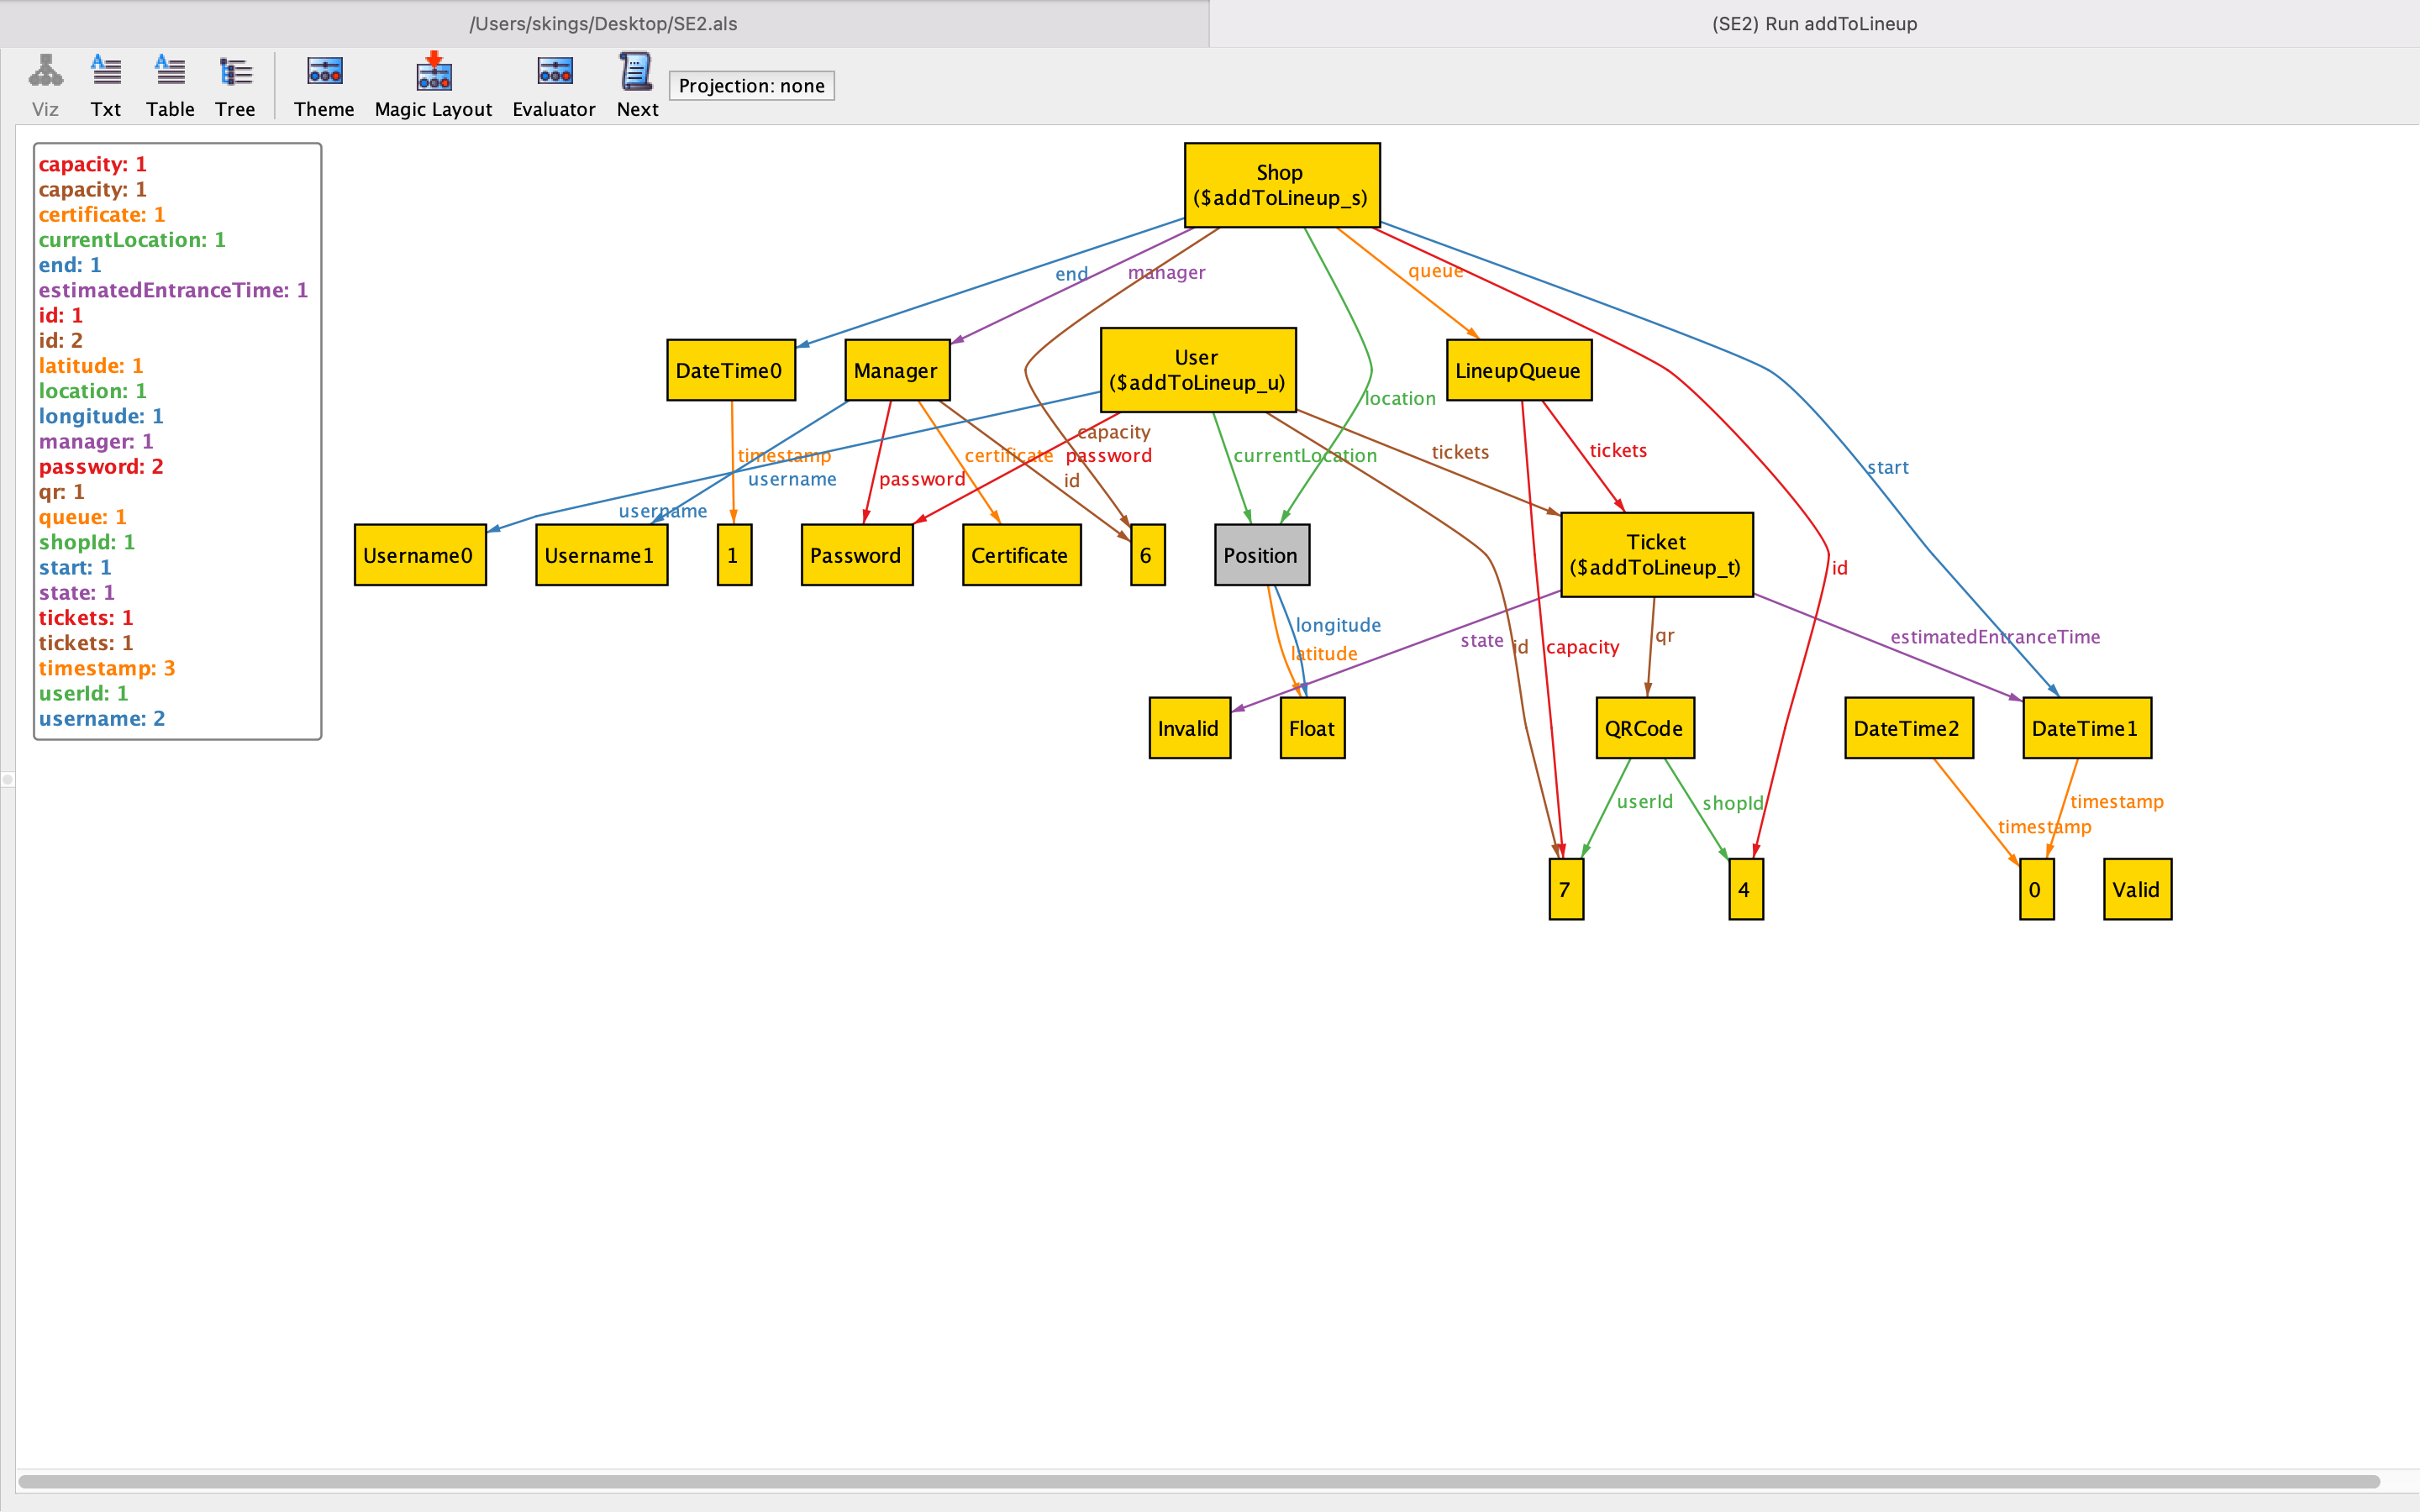
\includegraphics[width=0.9\textheight,keepaspectratio, angle=90]{images/alloy_addToLineup.png}
	\end{figure}
	\clearpage

	\item Book a visit \\
	\begin{figure}[H]
		\centering
		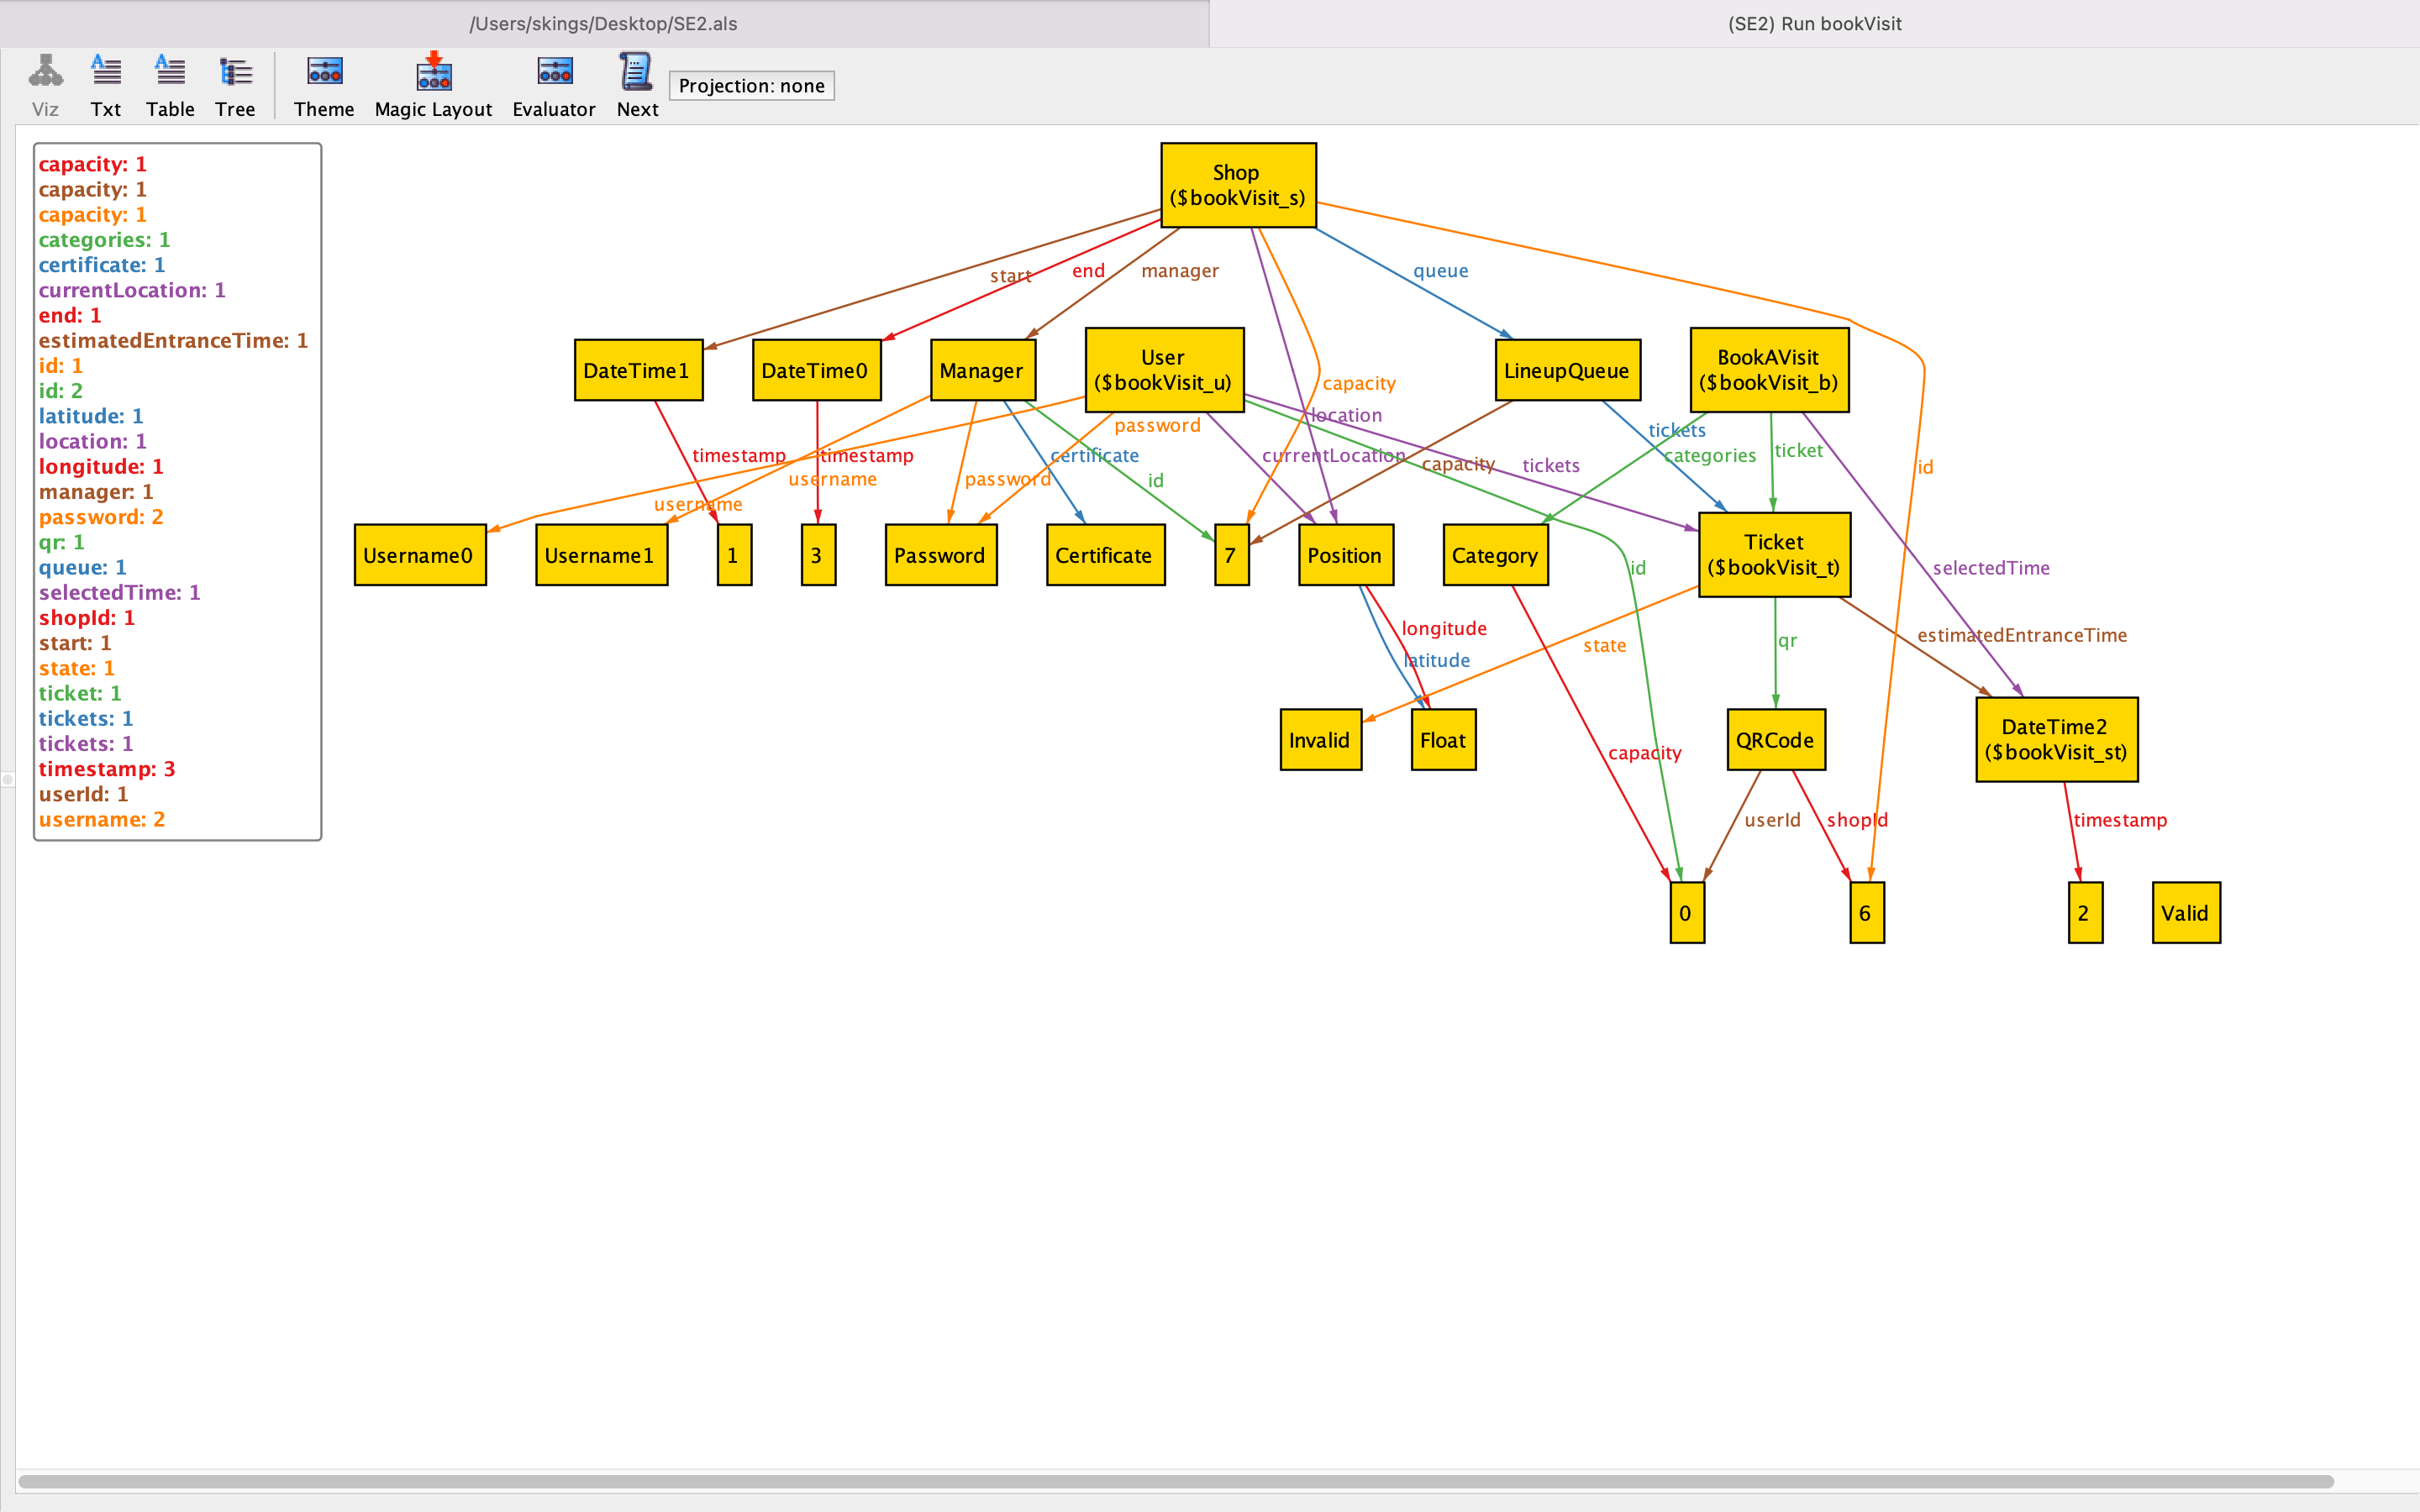
\includegraphics[width=0.9\textheight,keepaspectratio, angle=90]{images/alloy_BookVisit.png}
	\end{figure}
	\clearpage

	\item Get an offline ticket \\
	\begin{figure}[H]
		\centering
		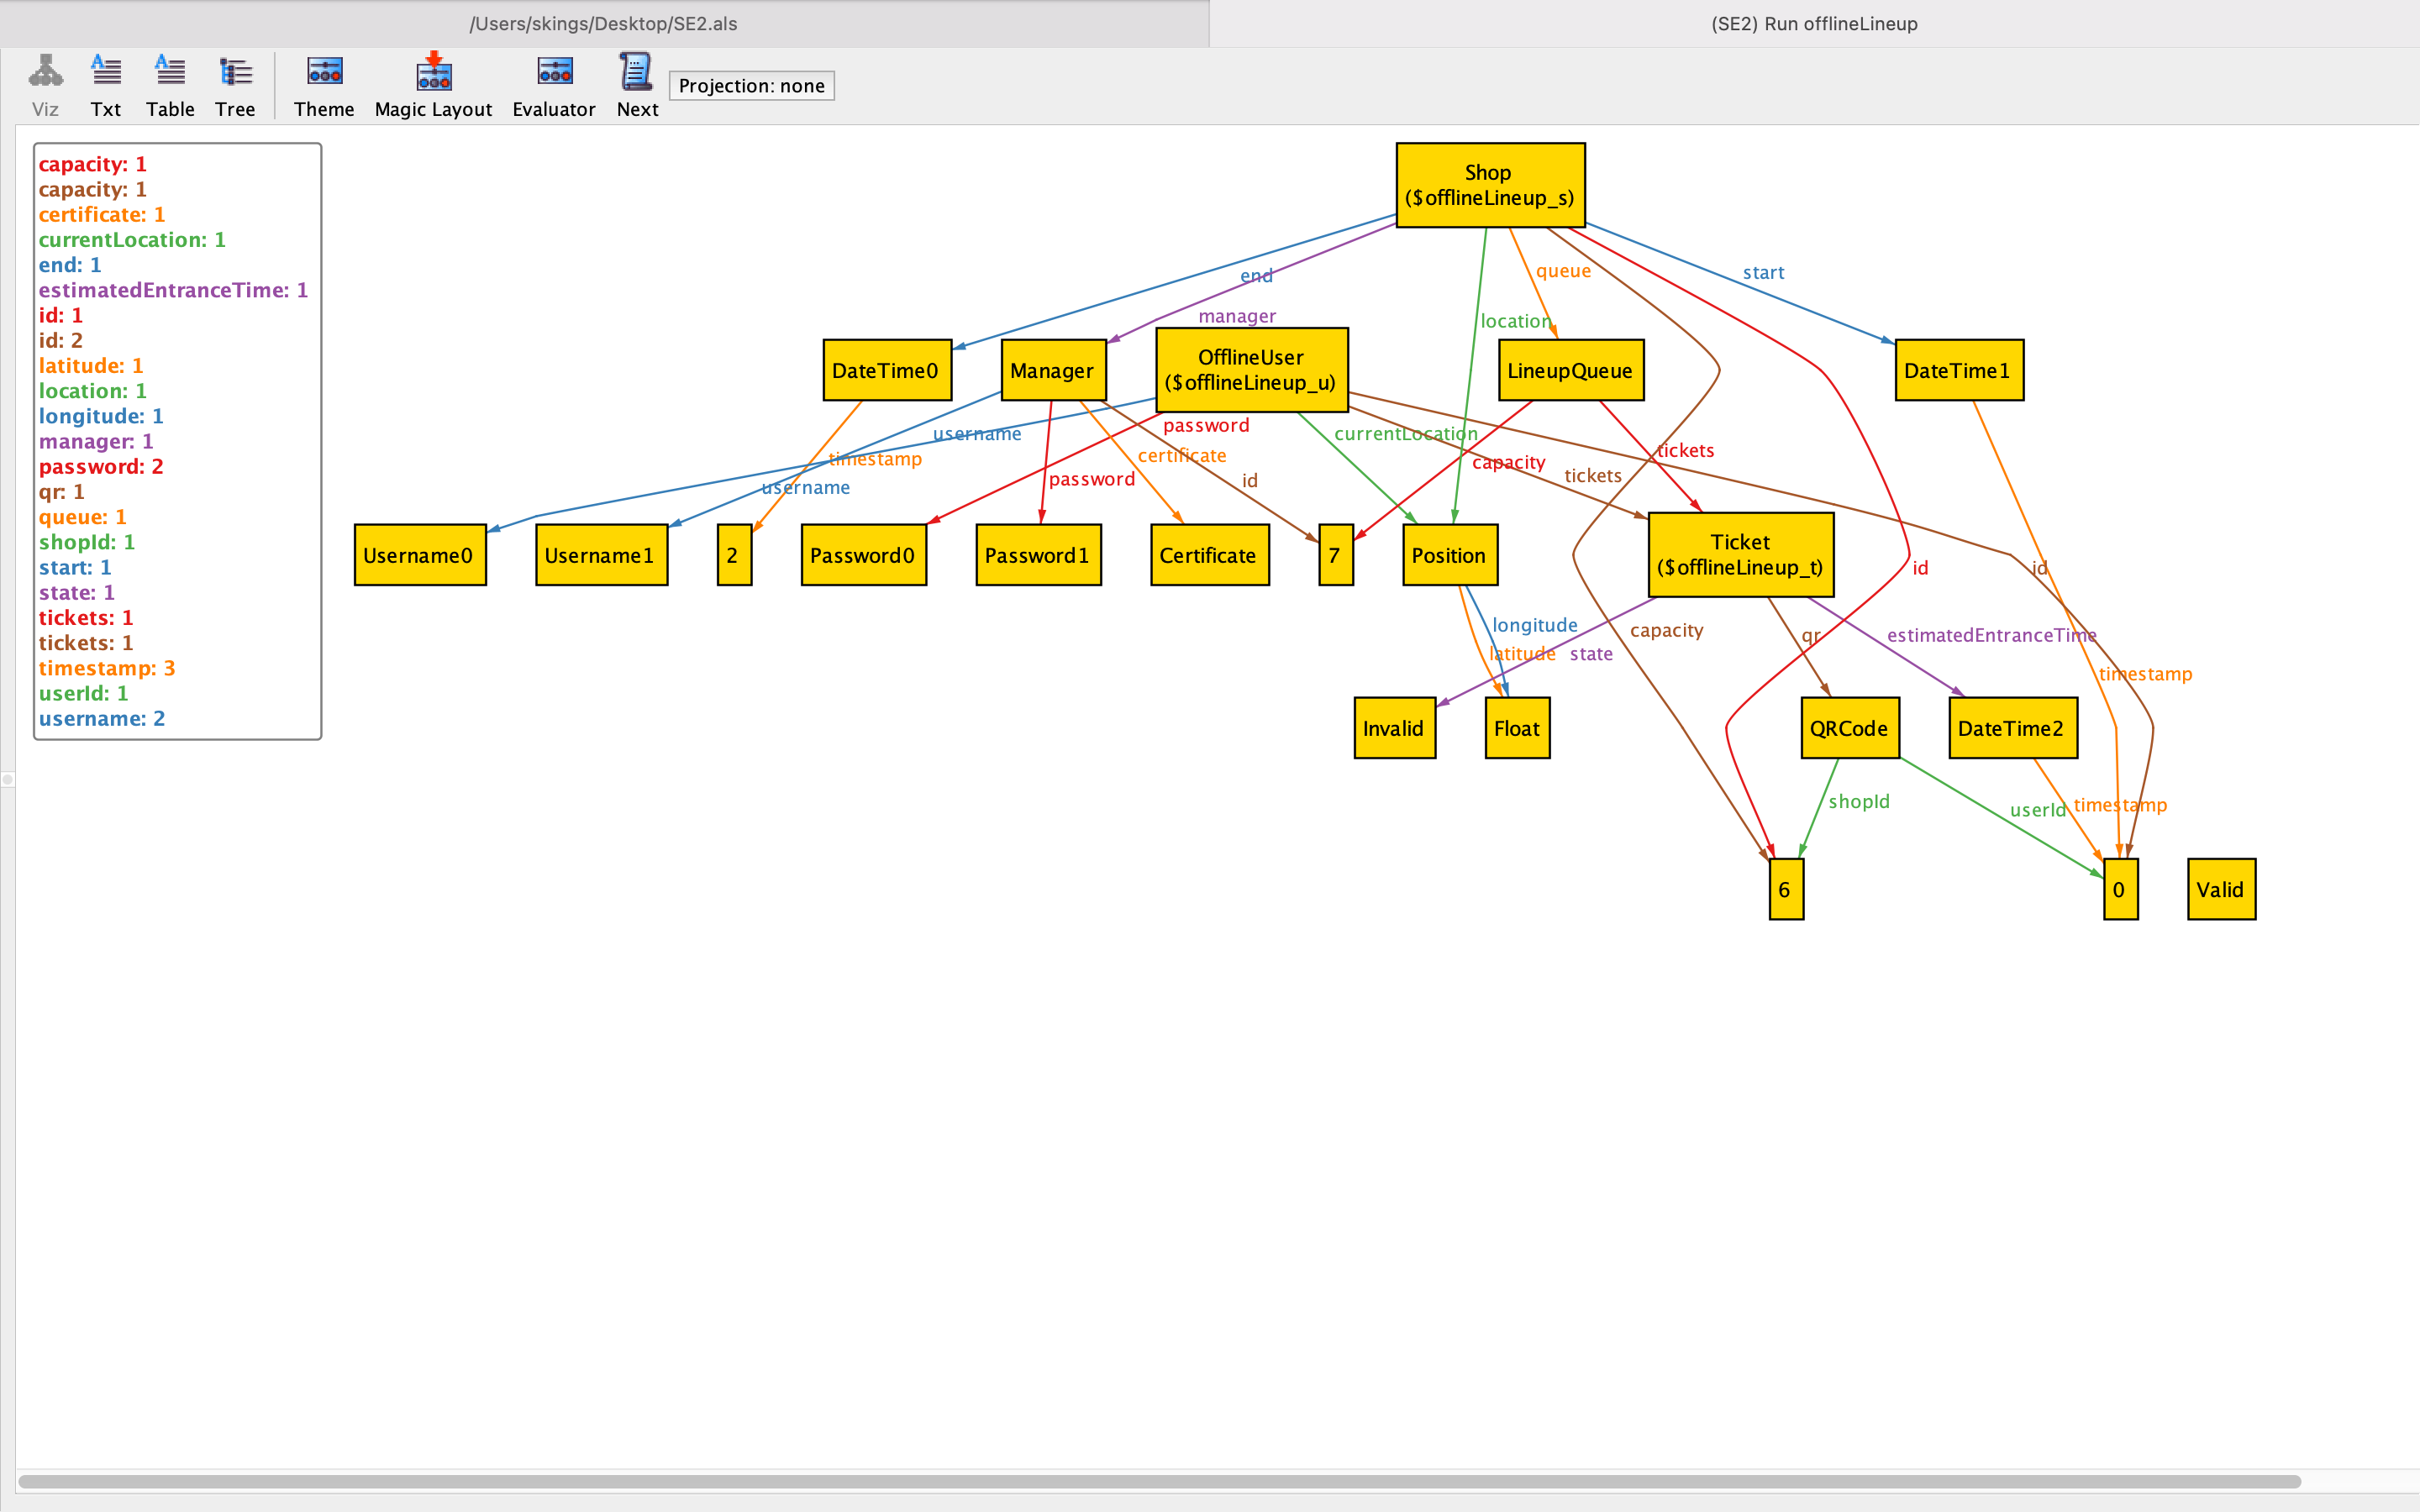
\includegraphics[width=0.9\textheight,keepaspectratio, angle=90]{images/alloy_OfflineLineup.png}
	\end{figure}
	\clearpage

	\item Allow Entrance \\
	\begin{figure}[H]
		\centering
		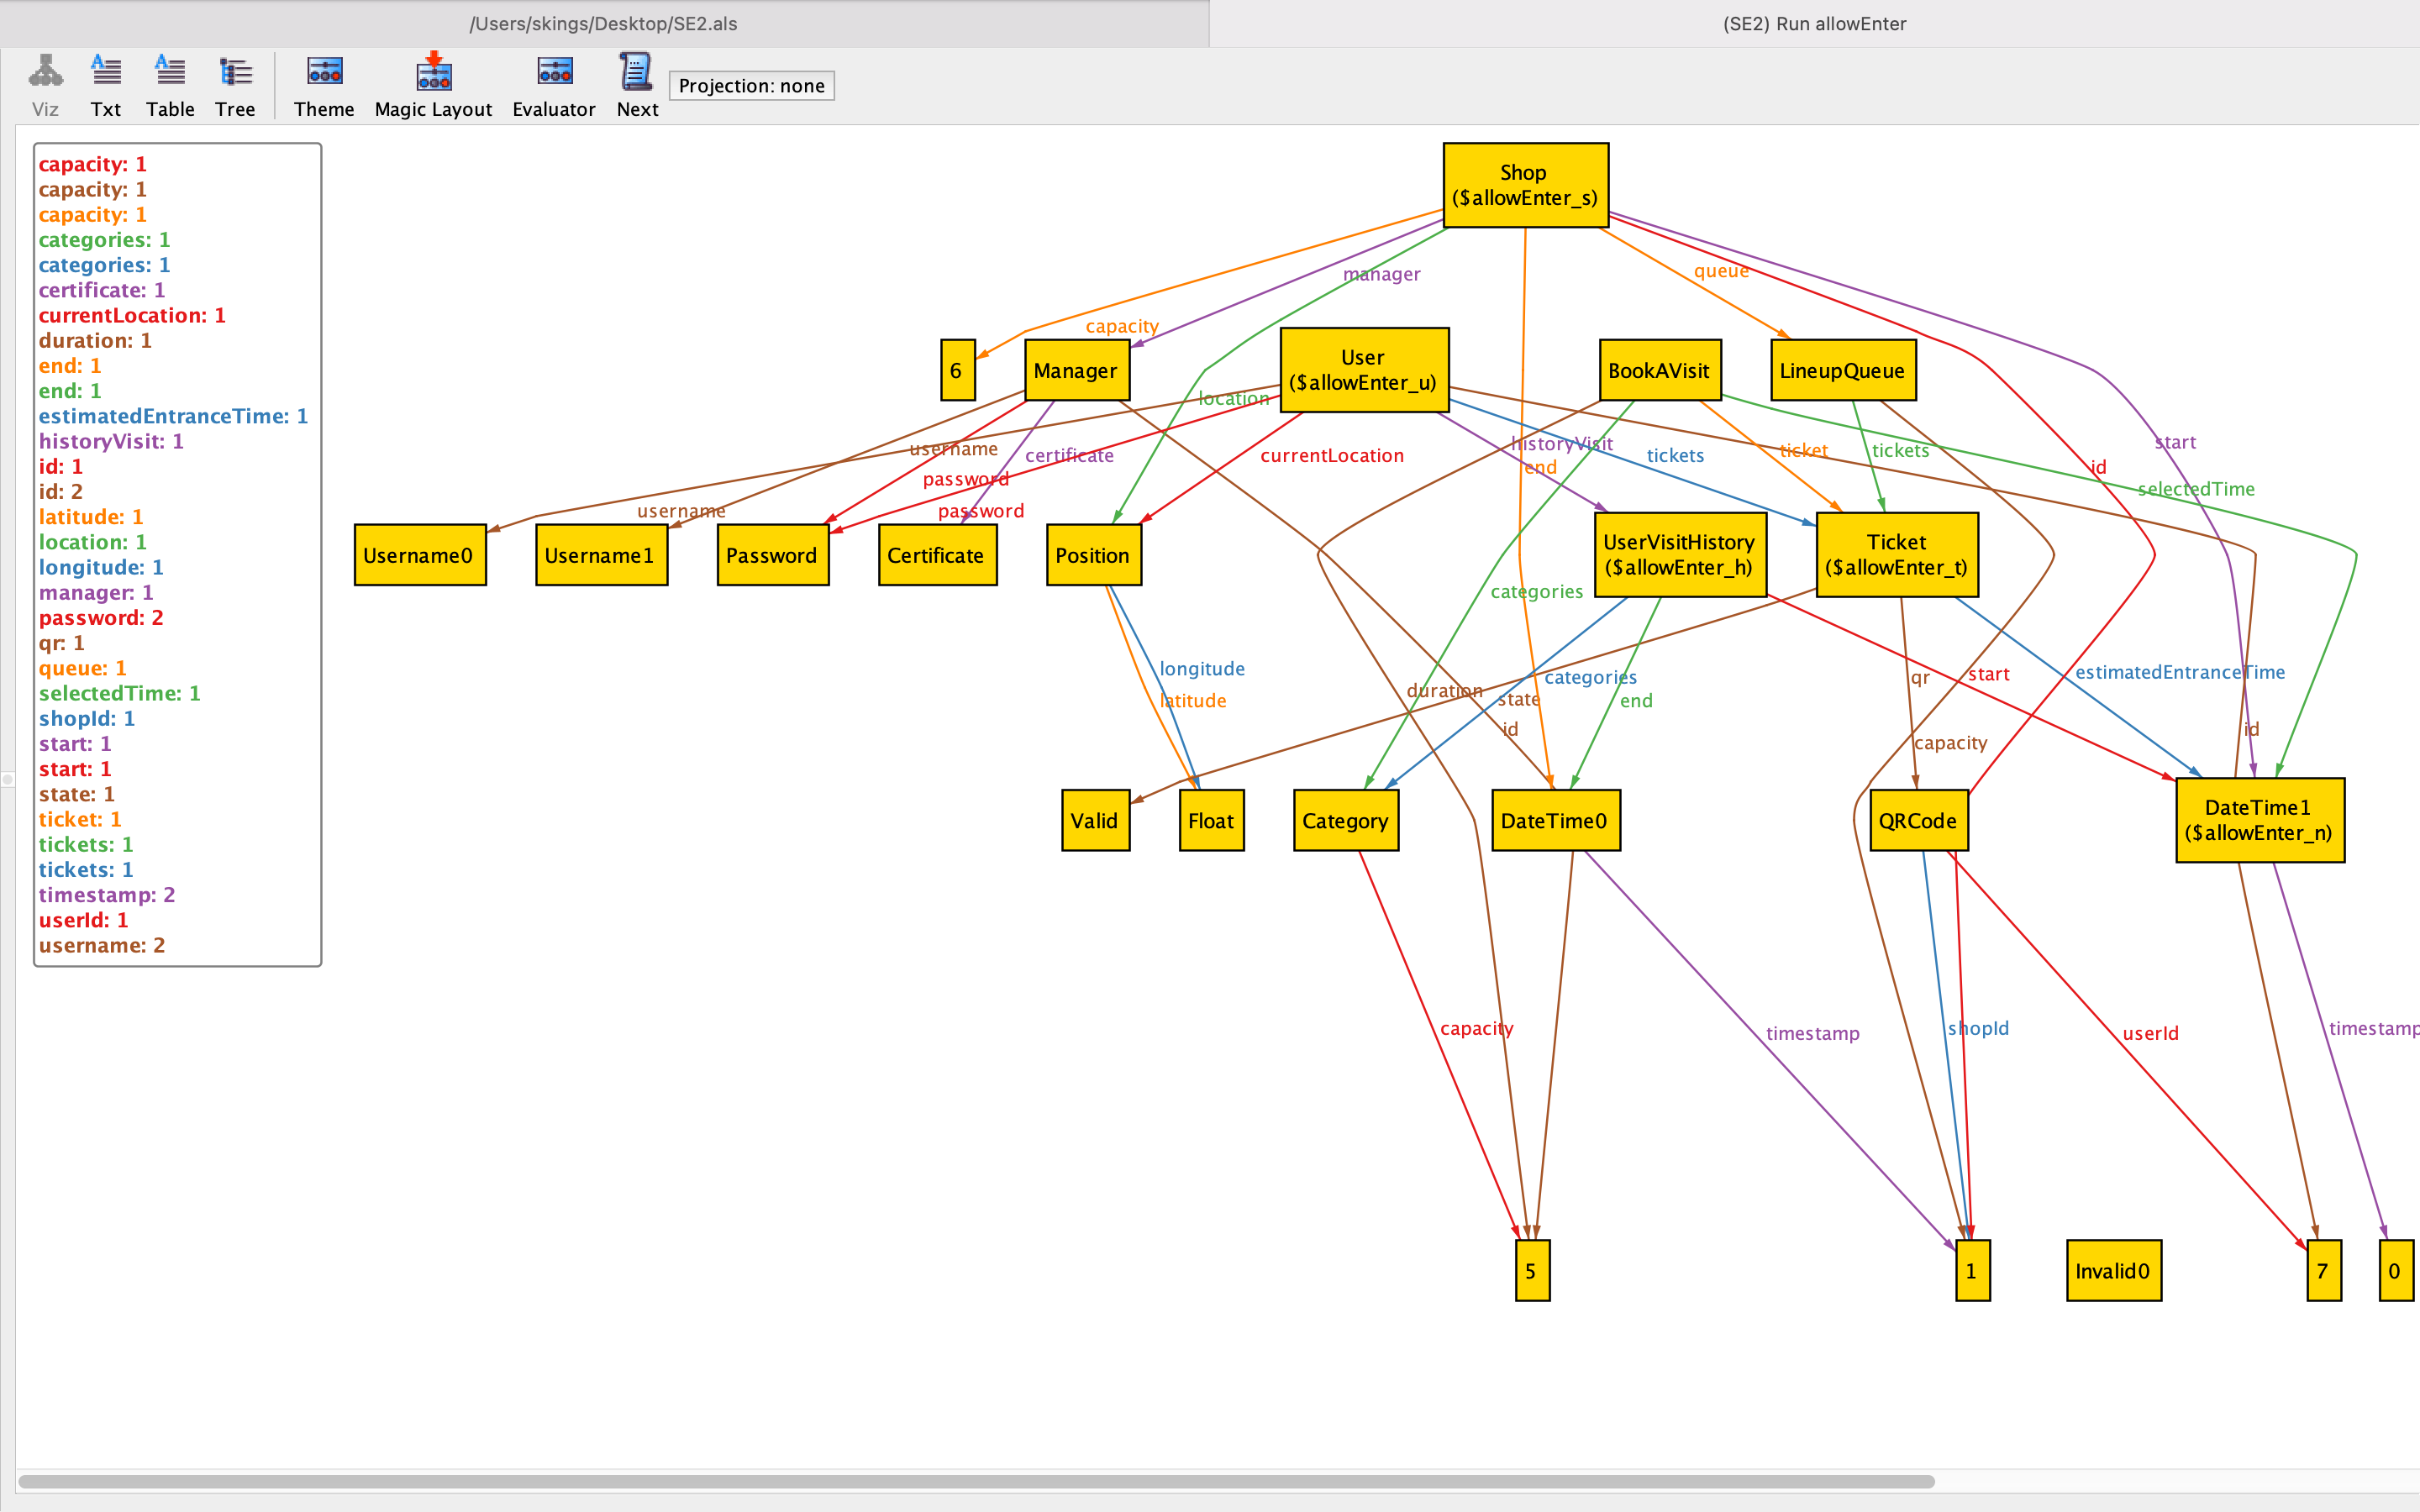
\includegraphics[width=0.9\textheight,keepaspectratio, angle=90]{images/alloy_AllowEnter.png}
	\end{figure}
	\clearpage

	\item Reject Entrance \\
	\begin{figure}[H]
		\centering
		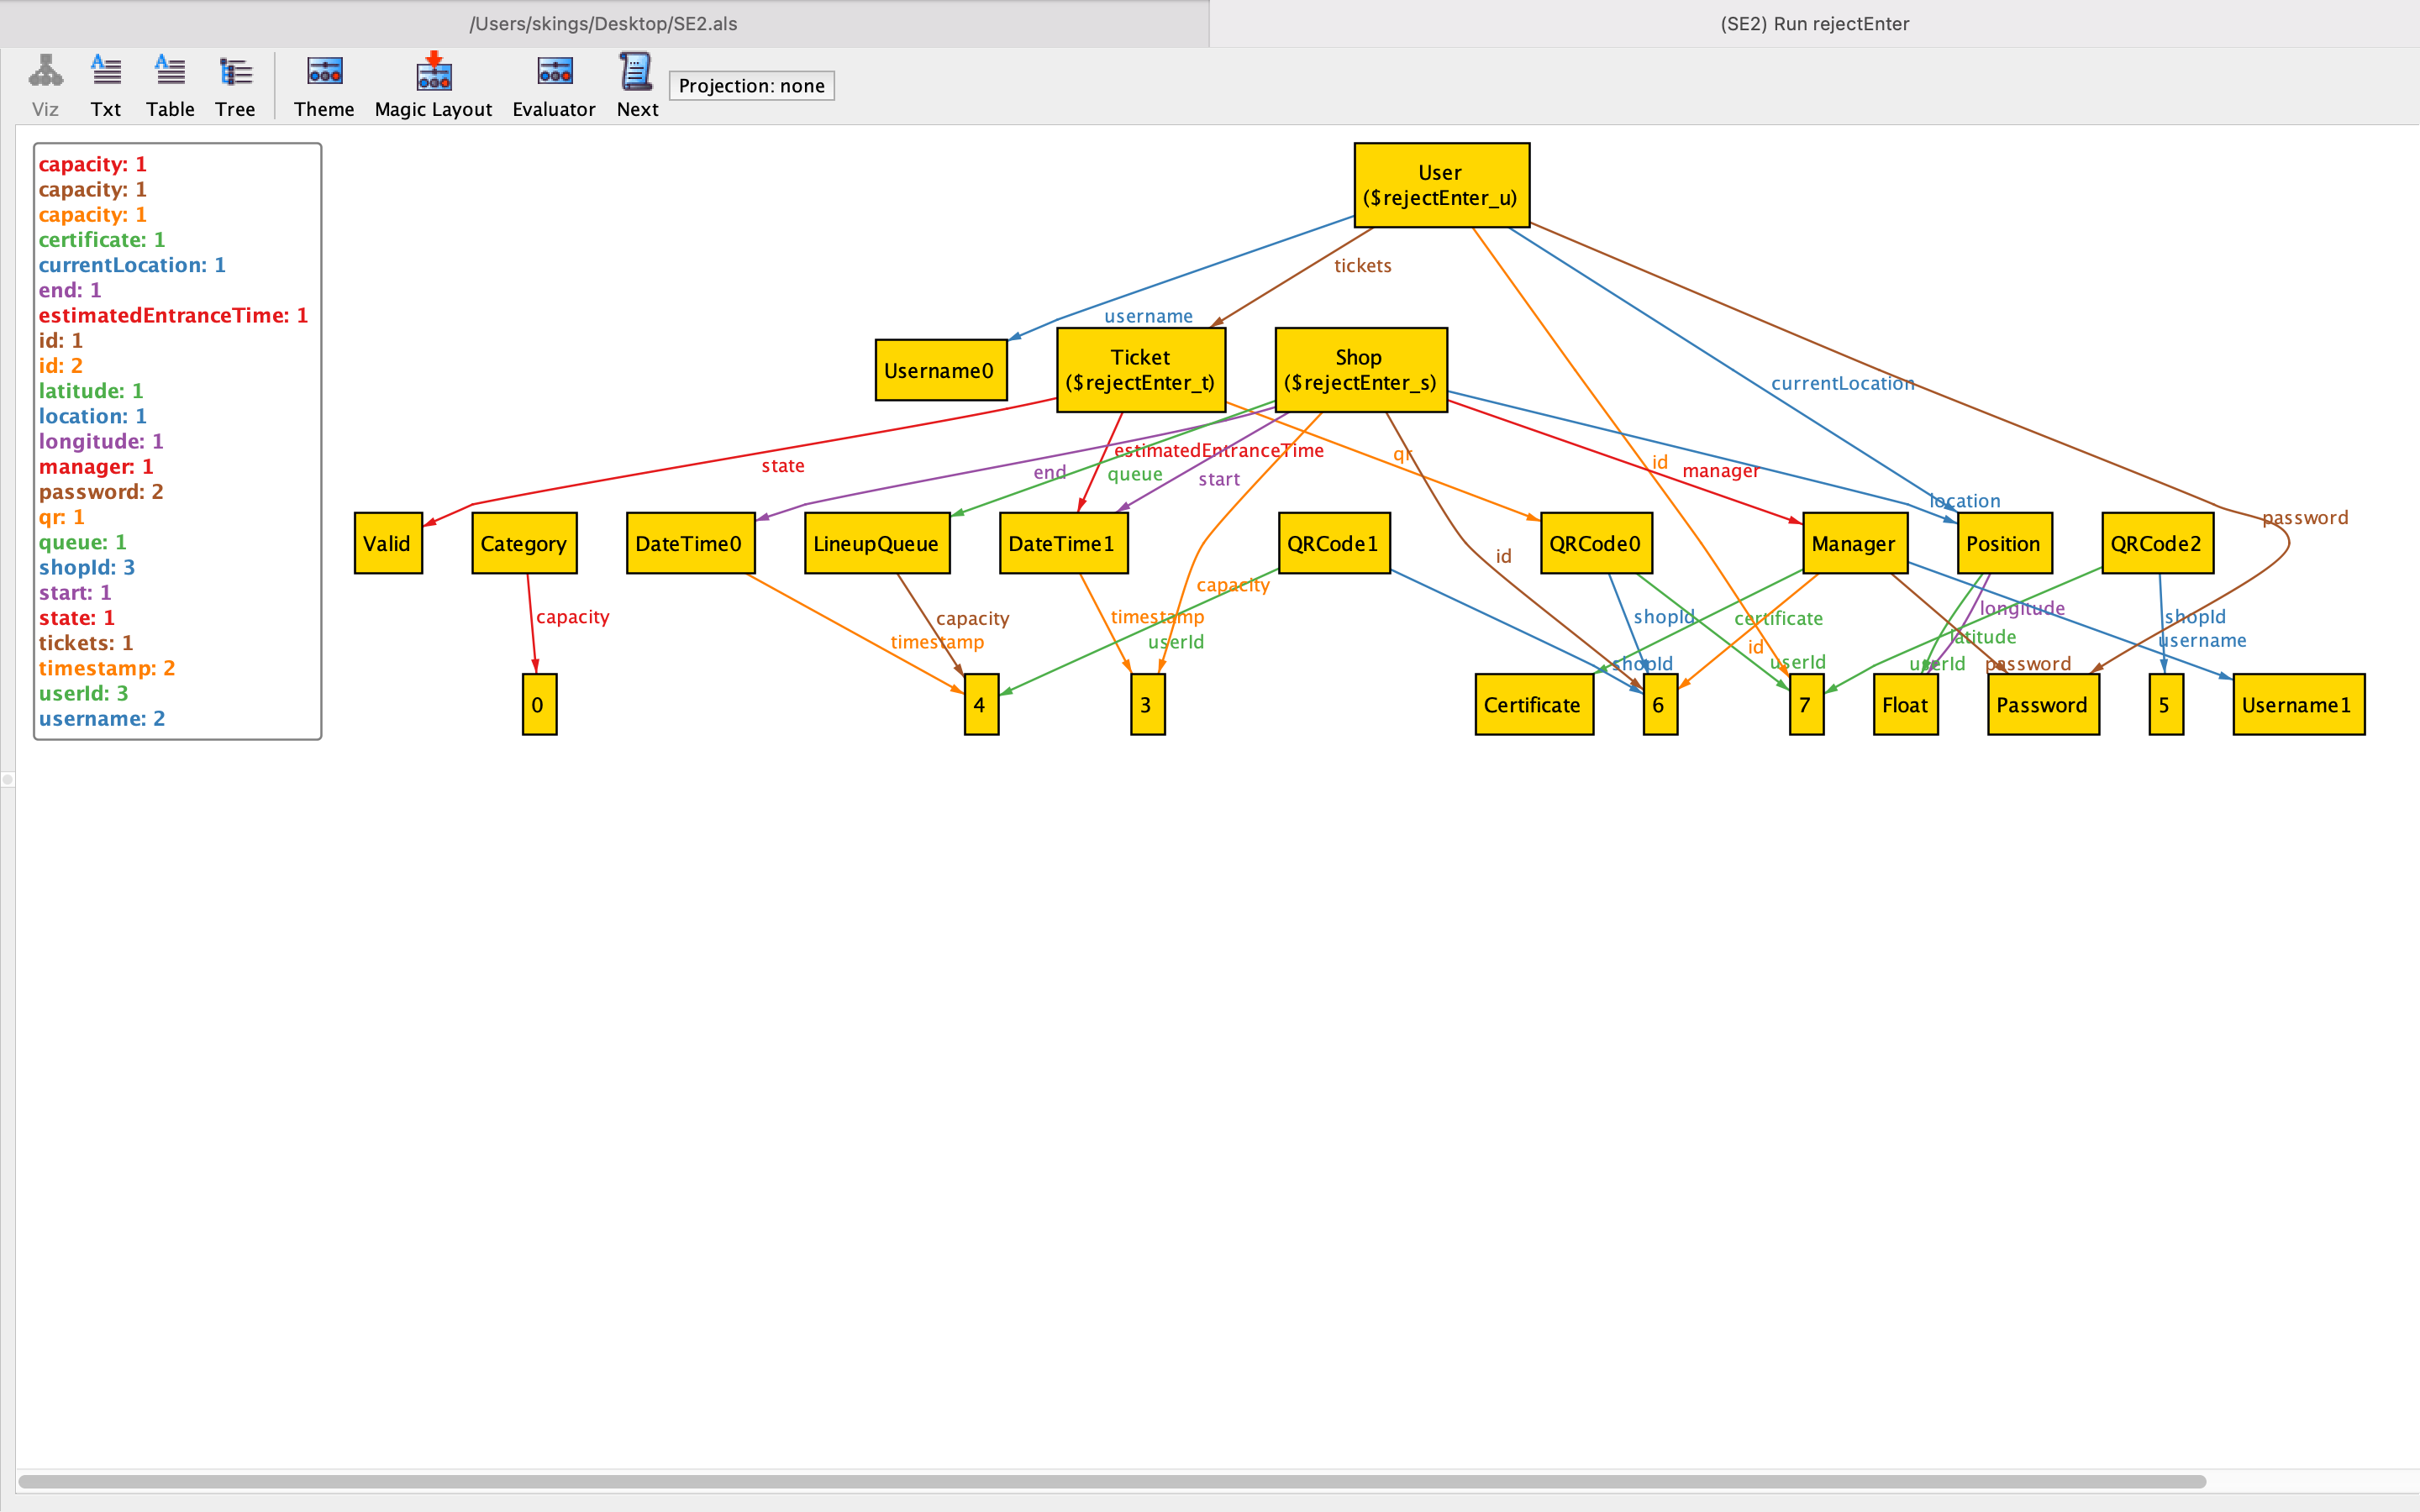
\includegraphics[width=0.9\textheight,keepaspectratio, angle=90]{images/alloy_rejectEnter.png}
	\end{figure}
	\clearpage

	\item Notify Entrance \\
	\begin{figure}[H]
		\centering
		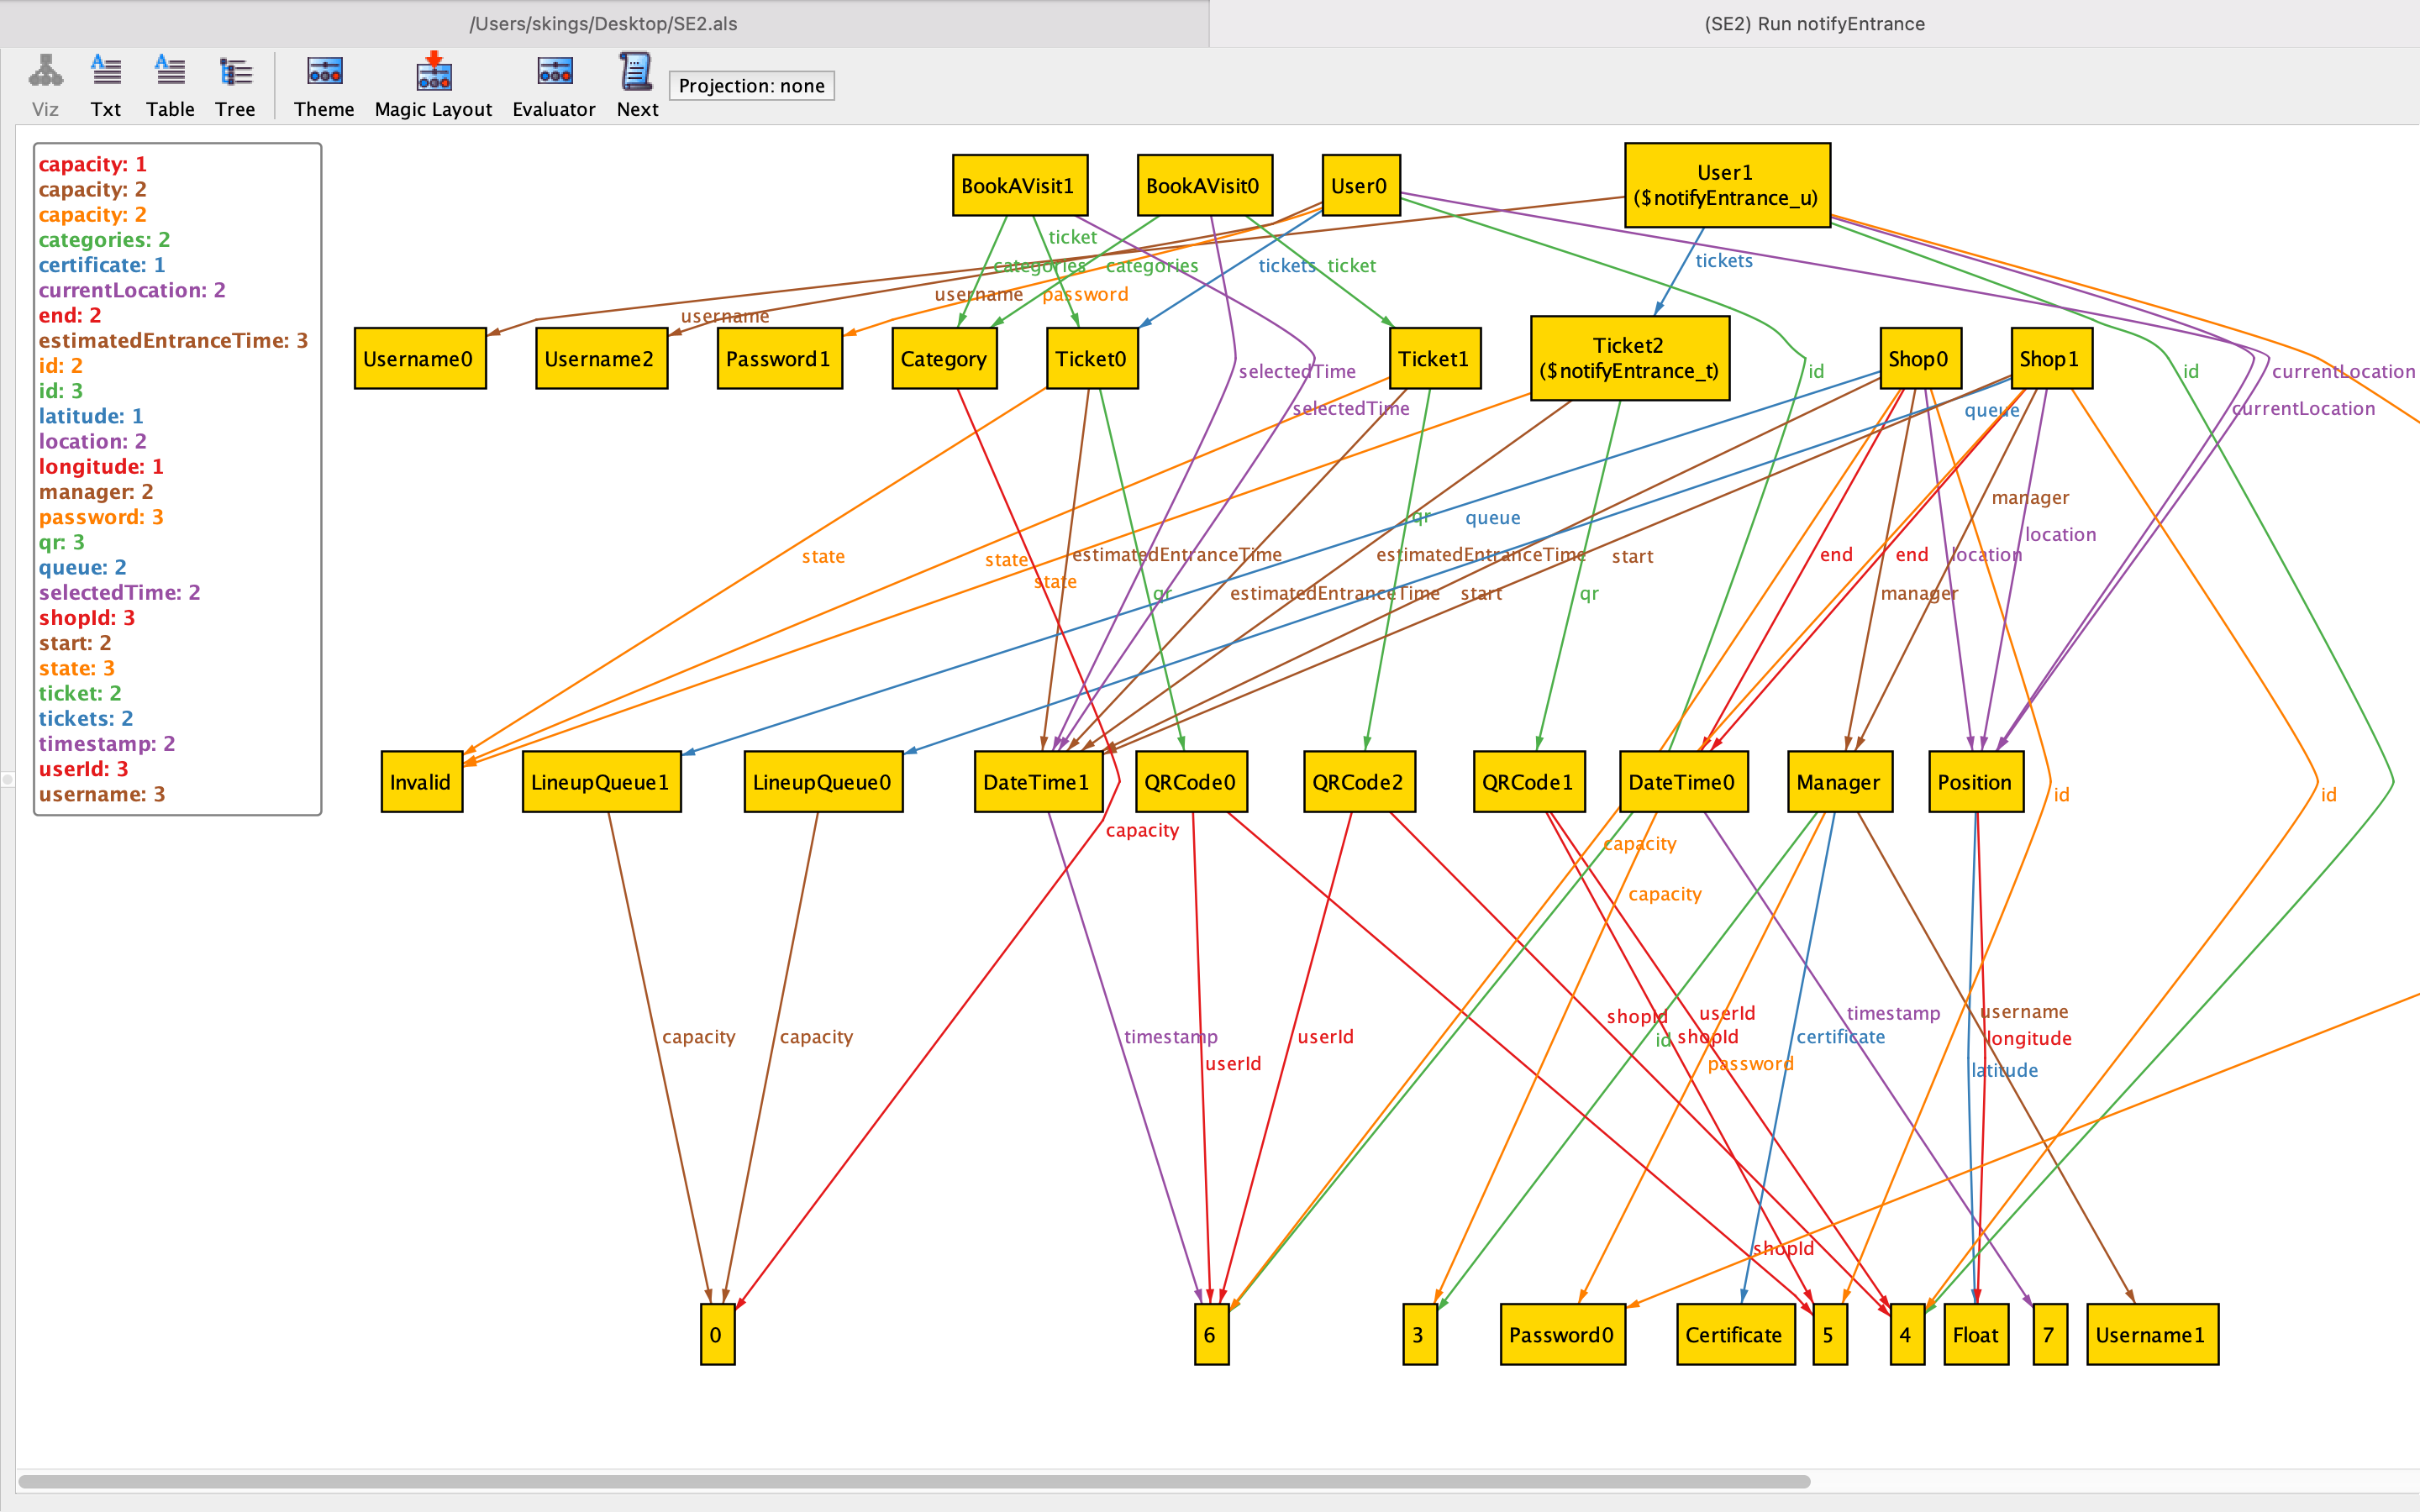
\includegraphics[width=0.9\textheight,keepaspectratio, angle=90]{images/alloy_notifyEntrance.png}
	\end{figure}
	\clearpage

	\item Checkout \\
	\begin{figure}[H]
		\centering
		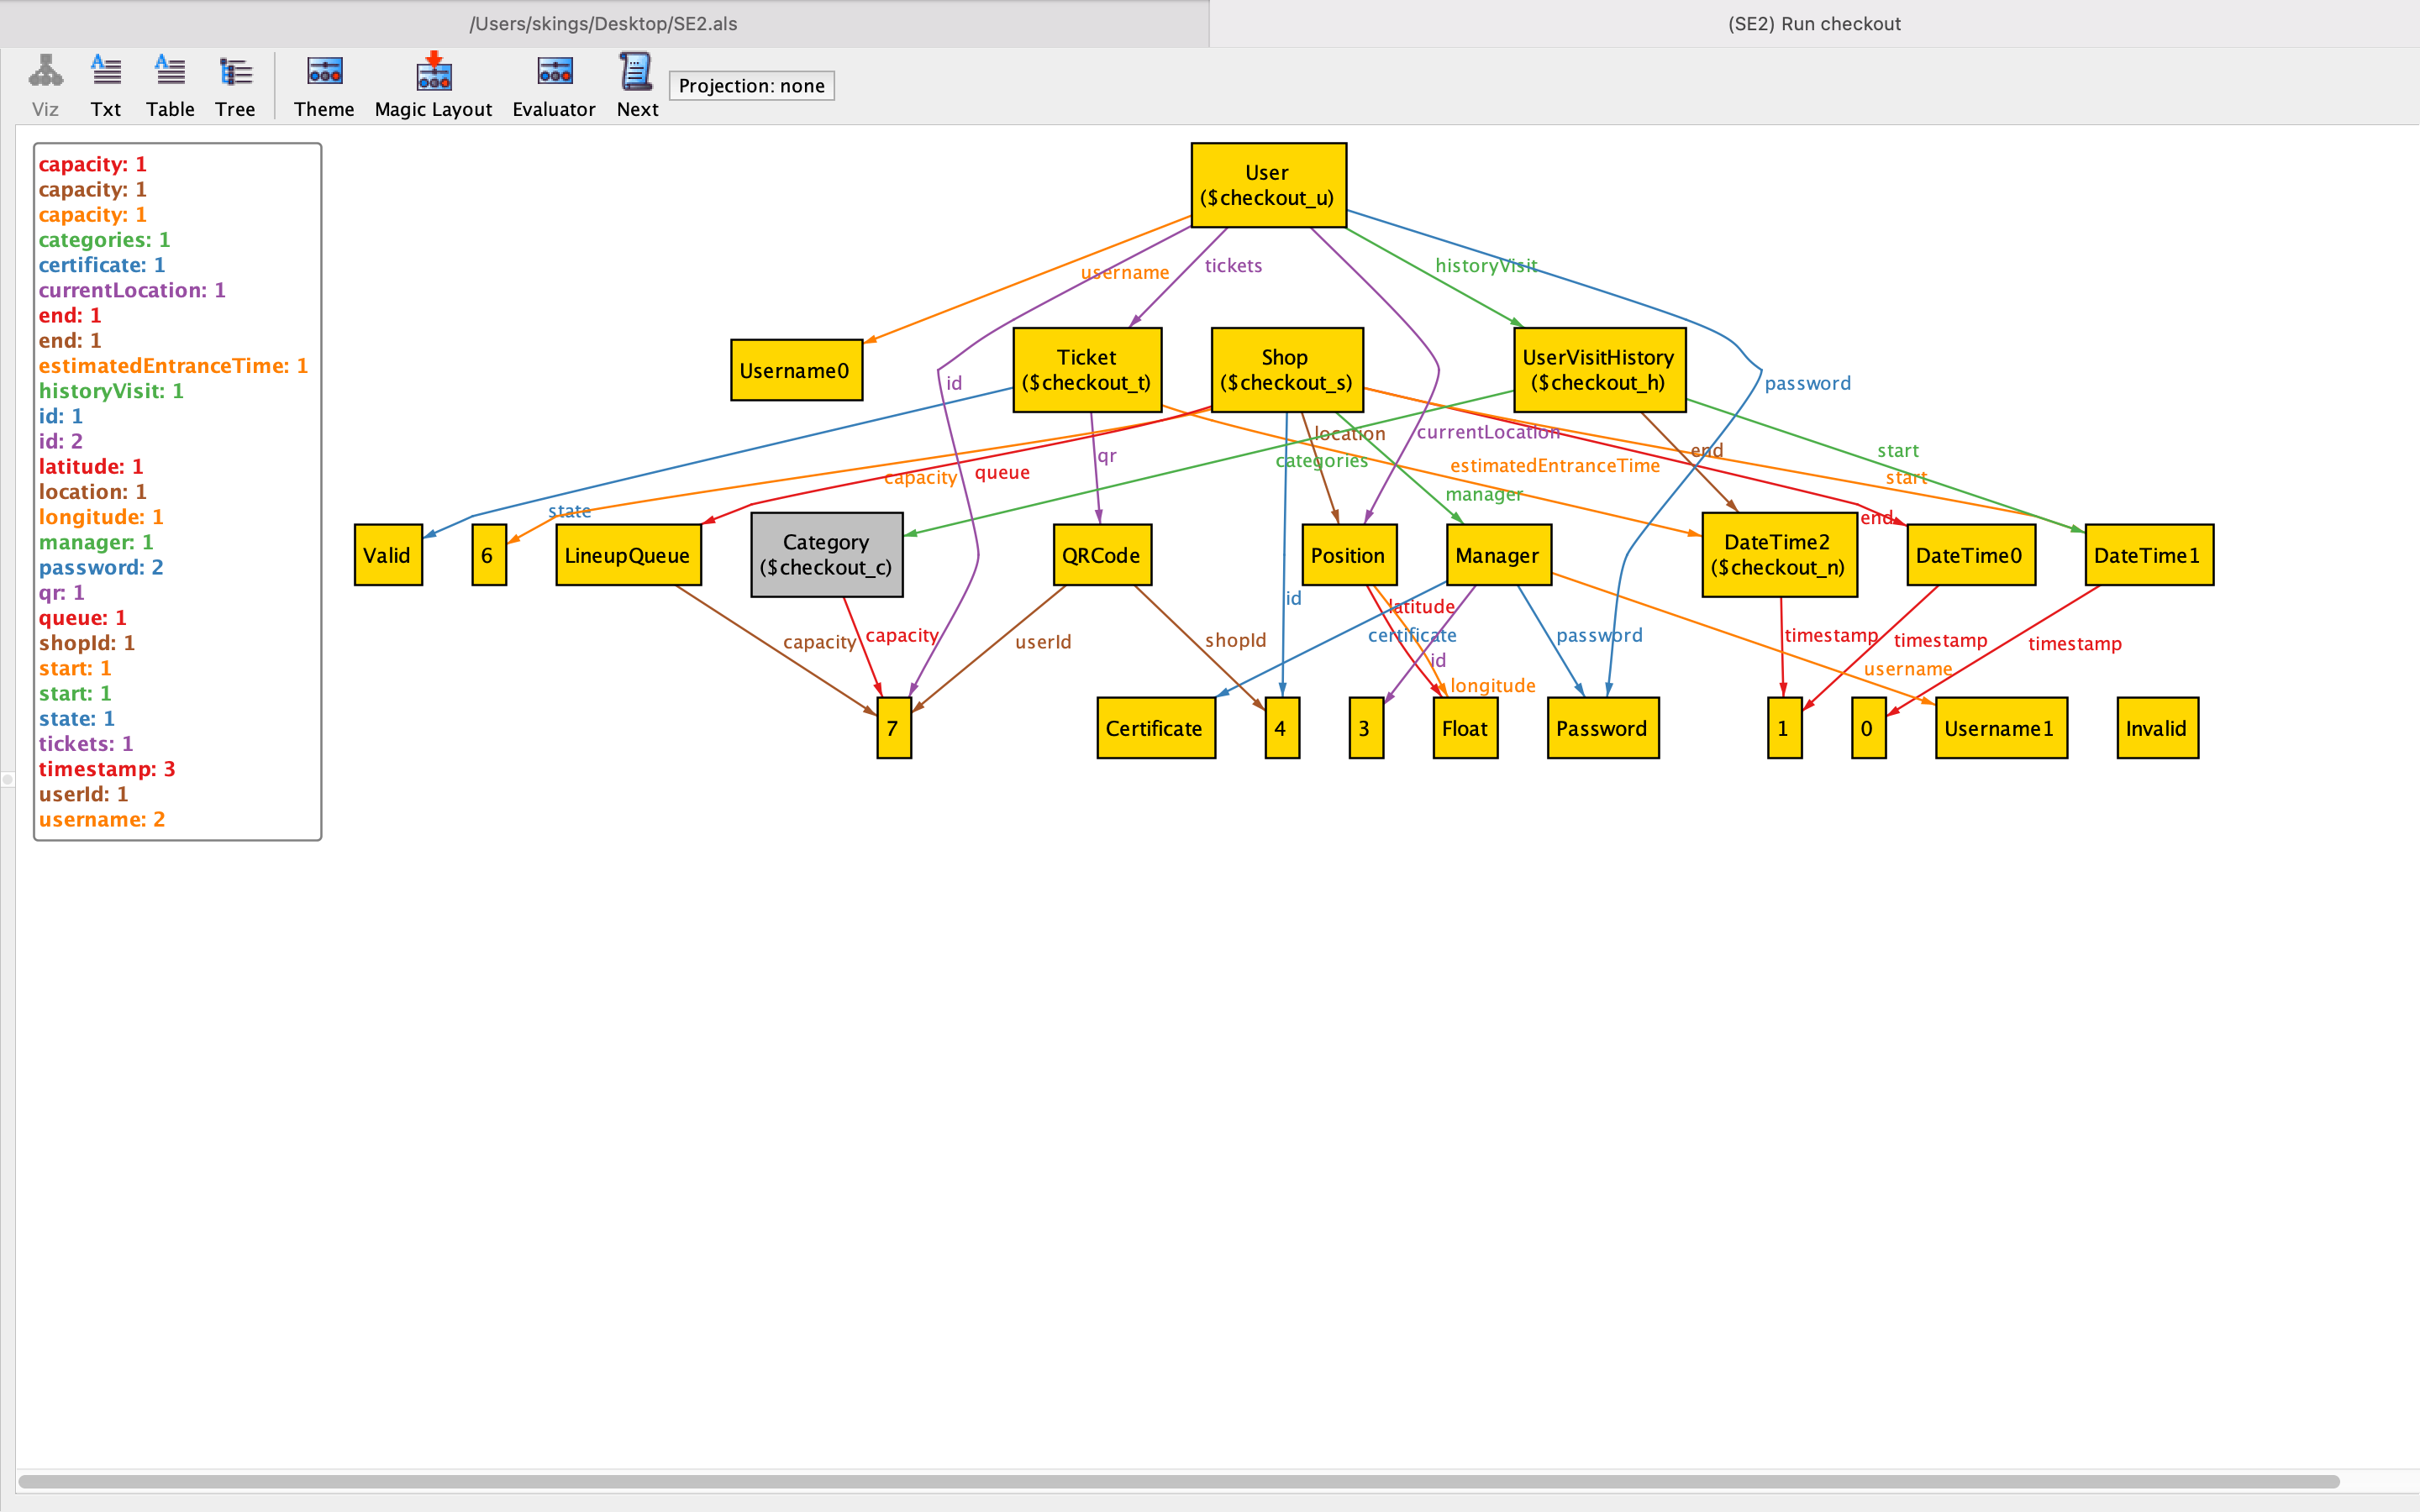
\includegraphics[width=0.9\textheight,keepaspectratio, angle=90]{images/alloy_checkout.png}
	\end{figure}
	\clearpage
\end{enumerate}


\section{Effort spent}

\section{References}
\end{document}
